\section{Experiments}\label{sec:experiments}
This section will describe our experiments and findings regarding utilizing context and graphs in recommender systems.
The section is structured as follows: First we will describe the state-of-the-art and baseline methods that have been investigated in \autoref{subsec:sotaoverview}.
We will then look at various datasets containing context, and briefly describe each of them in \autoref{subsec:desc-of-datasets}.
Following that we will look at various metrics used to evaluate recommender systems in \autoref{sec:evaluationmetrics}, and how these state-of-the-art methods compare to each other and baseline methods using these metrics in \autoref{subsec:resultsofexperiment}.

\subsection{State-of-the-art methods investigated}\label{subsec:sotaoverview}

\subsubsection{IS-UserBased-Graph}\label{method:IS-UserBased-Graph}
The \textit{IS-UserBased-Graph} method was first proposed by Tu Minh Phuong et. al in \cite{GraphBasedCollaborativePaper}.
As no implementation was available for this method , all results in later sections are based on our implementation.\\
The method utilizes a contextual modeling method called item splitting, in which each item is split into multiple fictional items to create a fictional item for each item and context variation.
For example, if we are considering the movie \textit{Die Hard}, and the contextual variable "watching with" which can have a value of either \textit{partner, family} or \textit{friends}, we will generate the following fictional items: \textit{(Die Hard, Partner)}, \textit{(Die Hard, Family)}, and \textit{(Die Hard, Friends)}.
Based on these fictional items, a bipartite graph is generated with the two sets $U$ for users and $I$ for fictional items, with each edge containing the rating that a user has rated a given fictional item.\\
To generate recommendations, the method utilizes a user similarity matrix to find the $N$ most similar users to the current user we are trying to generate recommendations for.\\
They present two ways to do this: Either by using matrix factorization or by using a spreading activation algorithm on the bipartite graph.
Both of these methods results in a list of the top-$N$ similar users, from which it is possible to estimate the missing rating $r_{ij}$ of the current user $u$ for a given item $i$,as seen on \autoref{eqn:israj}.
\begin{equation}
    \label{eqn:israj}
    r_{aj} = \frac{\sum_{R_{ij} \in R_j} r_{ij}}{|R_j|}, R_j = \{ r_{ij} | r_{ij} \neq \O , i \in u \}
\end{equation}
The method takes 2 parameters that influence the performance.
First is the \textit{L} value that indicates how many steps away from the current user you can move to calculate similarity by utilizing transitive associations, meaning that you take multiple steps away from the current node in a graph.
Second is the \textit{k} value which is the delimiter used for the \textit{kNN} algorithm in the next step.
After calculating the missing ratings, the last step is to map the fictitious items back to real items with their contextual information.
For example, if the fictional item \textit{(Die Hard, Family)} was the top recommendation, this would need to be mapped back to the movie Die Hard with the observed contextual variable \textit{watch with family}.\\
Finally, we apply post-filtering and remove all movies from the top-$N$ recommendations that do not fit the user's current context.\\
With this we now have a list of the top-$N$ recommended movies for the user $u$ in their given contextual situation.

\subsubsection{Context-Aware Matrix Factorization}\label{subsec:camf}
Another approach to CARS is \textit{context-aware matrix factorization} (CAMF)\cite{baltrunasCAMF}.
As no implementation was available for the method, all results are based on our implementation.
The method is an extension of the classical Matrix Factorization (MF) approach which takes the contextual side information into account when making rating predictions.
There are different models of \textit{CAMF} that deal with different levels of granularity in terms of the context.
For \textit{CAMF-C}, it is assumed that each of the contextual values has a global influence on the ratings independently of the items.
In the \textit{CAMF-C} model, a single parameter is introduced for each value of each contextual factor.
The second model is \textit{CAMF-CI} which introduces a parameter for each contextual value and item pair, meaning that it has a finer granularity.
By modelling it like this, it can capture when the contextual factors have a different effect on the rating depending on which item it is.
In this case, \textit{CAMF} is able to capture two different levels of granularity.
With \textit{CAMF-C}, for example, every movie will get an increased predicted rating across the board when it is raining outside as the contextual value.
For \textit{CAMF-CI}, however, only some specific movies will have their predicted ratings increased, while others may have their predicted ratings decreased when raining outside is used as the contextual value.
The expression for predicting ratings with the \textit{CAMF} models is seen in \autoref{eqn:camf-rating-pred}.
\begin{equation}
    \label{eqn:camf-rating-pred}
    \hat{r}_{uic_1...c_k} = \vec{v_u} * \vec{q_i} + \bar{i} + b_u + \sum\limits_{j = 1}^k B_{ijc_j}
\end{equation}
We have that $\hat{r}_{uic_1...c_k}$ is the predicted rating for user $u$ for item $i$ under the contextual values $c_1...c_k$.
The variables $\vec{v_u} $ and $ \vec{q_i}$ are the feature vectors for user $u$ and item $i$ which are multiplied.
This part is identical to what happens in matrix factorization, where the rating matrix is decomposed into the multiplication of two feature matrices, where one contains the features for each user and the other contains the features for each item.
$\bar{i}$ is the global average rating for item $i$ and $\bar{b_u}$ is a user bias. 
$B_{ijc_j}$ are the parameters modeling the interaction of the contextual conditions and the items.
For the \textit{CAMF-CI} model, $B_{ijc_j}$ will result in a lot of parameters, and for \textit{CAMF-C} it will result in less, as a result of how the two different approaches perform the contextual modeling.
All of the parameters in the model, except for the average item rating, are learned through stochastic gradient descent.
This is done through the use of the loss function seen in \autoref{eqn:camf-loss-func}.
\begin{equation}
    \label{eqn:camf-loss-func}
    \begin{split}
        \min_{v*, q*, b*, B*}\sum \limits_{r \in  R}\left [ \left (  \hat{r}_{uic_1...c_k} - \vec{v_u} * \vec{q_i} - \bar{i} - b_u - \sum\limits_{j = 1}^k B_{ijc_j}\right )^2 \right. \\
        \left. + \lambda \left({b_u}^2 +{\left \| \vec{v_u} \right \|}^2  + {\left \|\vec{q_i}  \right \|}^2 + \sum\limits_{j = 1}^k \sum\limits_{c_j = 1}^{z_j} B_{ijc_j}^{2}\right ) \right ]
    \end{split}
\end{equation}
Here we have that $r = (u,i,c_1...c_k)$ and $R$ is the context-dependent ratings from the training set.
$k$ is the number of different contextual factors and $z_j$ is the number of different contextual values for the contextual factor $j$.
The loss function includes regularization controlled by the $\lambda$ parameter to avoid overfitting the training data.
The parameters are then updated based on the gradient of the loss function for each of the ratings in the training set.

\subsubsection{Neural Graph Collaborative Filtering}\label{subsec:ngcf-desc}
\textit{Neural Graph Collaborative Filtering} (NGCF) is a method for collaborative filtering, employing a user-item bipartite graph structure.
Learnable collaborative filtering models contain two key components: embedding, which transforms users and items to representations, and interaction modeling, which reconstructs interactions based on these embeddings.
\textit{NGCF} aims to enhance recommendation by integrating user-item interactions into the embedding function, which has previously been built with descriptive features only, such as ID and attributes.
It does this through three components: an embedding layer that initializes user and item embeddings, embedding propagation layers that refine the embeddings, and a prediction layer aggregating the refined embeddings.
An initial embedding for a user $u$ is described as an embedding vector $e_u \in \R^d$, where $d$ is the embedding size.
Embeddings are propagated through two operations, construction and aggregation.
The embedding from item $i$ to user $u$ is defined in \autoref{eqn:ngcf-embed}:
\begin{equation}\label{eqn:ngcf-embed}
    m_{u \leftarrow i} = \frac{1}{\sqrt{|N_u||N_i|}} (W_1e_i + W_2(e_i \odot e_u))
\end{equation}
where $m_{u \leftarrow i}$ is the information to be propagated, $N_u$ and $N_i$ are the first-hop neighbors of user $u$ and item $i$, which are the neighbors that can be reached in one step from the node, $W_1, W_2 \in \R^{(d' \times d)}$ are trainable weight matrices, $d'$ is the transformation size and $\odot$ is the element-wise product.
The element-wise product ensures that the interaction between the embedding of item $i$ and user $u$ contributes to the result.
Aggregation for multiple layers is defined in \autoref{eqn:ngcf-agg}:
\begin{equation}\label{eqn:ngcf-agg}
    e_{u}^{(l)} = \textrm{LeakyReLU}(m_{u \leftarrow u} + \sum_{i \in N_u} m_{u \leftarrow i})
\end{equation}
where $e_u^{(l)}$ is the representation of $u$ obtained at the layer and LeakyReLU is the activation function.
The information being propagated, $m_{u \leftarrow i}$ and $m_{u \leftarrow u}$ is defined in \autoref{eqn:ngcf-userrep}:
\begin{equation}\label{eqn:ngcf-userrep}
  \begin{cases}
    m_{u \leftarrow i}^{(l)} = \frac{1}{\sqrt{|N_u||N_i|}} (W_1^{(l)} e_i^{(l-1)} + W_2^{(l)} (e_i^{(l-1)} \odot e_u^{(l-1)}))\\
    m_{u \leftarrow u}^{(l)} = W_1^{(l)}e_u^{(l-1)}
  \end{cases}
\end{equation}
where $W_1^{(l)}$ and $W_2^{(l)}$ once again are trainable matrices, and $e_i^{(l-1)}$ is the item representation generated the the previous layer.
After $L$ layers of propagation there are multiple representations for user $u$, ${e_u^{(1)},...,e_u^{(L)}}$. These representations are concatenated for the final representation, meaning each corresponding entry in the different embeddings are combined for the final embedding, and the same operation is performed on the item representations.
Finally, the inner product is calculated between the user and given item representation, as shown in \autoref{eqn:ngcf-predict}:
\begin{equation}\label{eqn:ngcf-predict}
  \hat{y}(u, i) = e_U^{*^\textrm{T}} e_i^*
\end{equation}
where $*$ is used to denote the final concatenated representation of the user and the item.
Learning model parameters with \textit{NGCF} is done through optimizing the pairwise Bayesian Personalized Ranking (BPR) loss.
BPR assumes that observed interactions should be assigned higher prediction values than unobserved ones since these are more reflective of preferences.
The objective function is defined in \autoref{eqn:ngcf-loss}.
\begin{equation}\label{eqn:ngcf-loss}
    Loss = \sum_{(u, i, j) \in O} - \textrm{ln} \: \sigma (\hat{y}_{ui} - \hat{y}_{uj}) + \lambda ||\Theta||_2^2
\end{equation}
where $O = {(u, i, j) | (u, i) \in R^+, (u, j) \in R^-}$, where $i$ and $j$ are items from respectively observed interactions $R^+$ and unobserved interactions $R^-$, $\sigma$ is the sigmoid function, $\Theta$ denotes all trainable model parameters and $\lambda$ is a regularization parameter.
\textit{NGCF} employs dropout to avoid overfitting in neural networks.
\textit{NGCF} randomly drops information being propagated through \autoref{eqn:ngcf-userrep} by a probability, as well as dropping nodes in training by randomly blocking and discarding all its outgoing information.

\subsubsection{LightGCN}
In \cite{LightGCN}, Xiangnan He et. al investigated the \textit{NCGF} method by exploring the effects that the nonlinear activation function and feature transformation had on the model's results.
They found that by removing these parts of the \textit{NGCF} model they were able to achieve better results, meaning that these parts negatively affected the training of the model.
Inspired by this, Xiangnan He et. al came up with a light but effective model of a graph convolutional network (GCN) with only the most essential parts used for collaborative filtering called \textit{LightGCN}.
For the experiments, we use the official TensorFlow based implementation of the paper available on \href{https://github.com/kuandeng/LightGCN}{GitHub}.
Like \textit{NGCF}, this method produces implicit ratings in the form of a top-$N$ list.
\\\\
The idea of a GCN is to learn the representation of nodes by smoothing features over the graph \cite{LightGCN}.
This is done by performing graph convolution where features of neighboring nodes are aggregated to give a new representation of the target node.
They propose an aggregation function called Light Graph Convolution (LGC) seen in \Cref{eqn:lgc}.
\begin{align}\label{eqn:lgc}
    e_{u}^{(k+1)}=\sum_{i\in N_u}\frac{1}{\sqrt{\left | N_u \right |}\sqrt{\left | N_i \right |}}e_{i}^{(k)},\nonumber\\
    e_{i}^{(k+1)}=\sum_{u\in N_i}\frac{1}{\sqrt{\left | N_i \right |}\sqrt{\left | N_u \right |}}e_{u}^{(k)}
\end{align}
$e_{u}^{(k+1)}$ and $e_{i}^{(k+1)}$ are the embeddings at layer $k+1$ for a user $u$ and item $i$ respectively.
$N_u$ are the items that user $u$ has interacted with and $N_i$ are the users that have interacted with item $i$.
Note that this aggregation does not contain any nonlinear activation function nor any feature transformation, unlike NGCF's aggregation function described in \Cref{eqn:ngcf-agg}.
$\frac{1}{\sqrt{\left | N_u \right |}\sqrt{\left | N_i \right |}}$ is a symmetric normalization term which makes sure that the embeddings do not scale with increasing graph convolution operations.
In LGC the target node is not included in the aggregation and only the neighboring nodes are used which means that it does not handle self-connections.
This is instead handled in a later operation where the layers are combined.
\\
The only trainable model parameters in \textit{LightGCN} are the embeddings at the 0-th layer which are $e_{u}^{(0)}$ for the users and $e_{i}^{(0)}$ for the items.
Embeddings at higher layers are computed using the LGC aggregation function. 
When the embeddings at the final layer have been computed, layers are combined through a summation to get a final presentation of the users and items.
\begin{align}\label{eqn:lgcn-layer-comb}
    e_{u} = \sum_{k=0}^K \alpha_k e_{u}^{(k)} \nonumber\\
    e_{i} = \sum_{k=0}^K \alpha_k e_{i}^{(k)}
\end{align}
In \Cref{eqn:lgcn-layer-comb} we have $\alpha_k \geq 0$ which is a weight that indicates the importance of the embedding on layer $k$.
They found that setting this parameter to $1/(K+1)$ uniformly led to a good performance, but the parameter can be learned as a model parameter.
There are a few reasons why the layer combination is a good thing to do.
\\
First of all, the embeddings become over-smoothed with an increasing number of layers, meaning that the embeddings slowly become indistinguishable when too much graph convolution is done.
This may be avoided by combining the embeddings at the different layers in the final step of the model.
Secondly, the embeddings at the different layers capture different features that would not be expressed if only the last layer's embeddings were used for the final embeddings.
For example, aggregation at the first layer captures the direct interactions between users and items, the second layer captures users that have an overlap in their item interactions, and so on.
Finally, when the embeddings at different layers are combined with a weighted sum, the effect of graph convolution with self-connections is captured.
\\
After the layer combination, the final embeddings can be used to make predictions with the model as seen in \Cref{eqn:lgcn-pred}.
\begin{align}\label{eqn:lgcn-pred}
    \hat{y}_{ui} = e_U^{*^\textrm{T}} e_i^*
\end{align}

\subsubsection{KGAT}
Knowledge Graph Attention Network for Recommendation (KGAT) was proposed by Xiang Wang et. al in \cite{KGAT}.
The main contribution for KGAT is the ability to model side information, such as item attributes and context while taking high-order connectivity into account by utilizing a collaborative knowledge graph (CKG).
This collaborative knowledge graph is presented as an extension to the bipartite graph with the two distinct sets $U$ and $I$ indicating respectively users and items.
In addition to the bipartite graph, we have a knowledge graph containing side information for items, where an interaction between users $U$ and items $I$ is described as a tuple $(u, r, i)$ indicating that a user $u \in U$ has a relation $r$ to an item $i \in I$.
These two are combined as a CKG where we represent a user behavior triplet as $(u, Interact, i)$ to indicate an interaction between $u$ and $i$, by unifying the two graphs as $G = \{(u, r, i) | u, i \in E, r \in R\}$ where E is the set of entities describing side-information and R is the set of possible relations between entities.\\
Finally, KGAT utilizes high-order connectivity to increase recommendation quality.
The \textit{L-order connectivity} between nodes is defined as a multi-hop relational path between entities: $e_0 \overset{r_1}{\rightarrow} e_1 \overset{r_2}{\rightarrow} \dots \overset{r_L}{\rightarrow} e_L$ where $e_l \in E$, $r_l \in R$ and $l \in L$.
In a real world scenario, this could look like: $u_1 \overset{r_1}{\rightarrow} i_1 \overset{-r_1}{\rightarrow} u_2 \overset{r_1}{\rightarrow} i_2$ suggesting that $u_1$ would be interested in $i_2$ since their similar user $u_2$ has expressed interest in $i_2$.
The relations $r$ are arbitrary directed relations, and a negative relation $-r$ indicates going against the direction.
Additionally, KGAT allows us to model relations based on entities across different relation types, for example if $u_1$ likes movies with Bruce Willis as an actor, they may also like movies produced by him.
\\
The methodology for doing this consists of three main components: An embedding layer, an attentive embedding propagation layer, and a prediction layer.\\
For an overview, the embedding layer handles mapping entities and their relations into a lower dimension space.
The attention embedding propagation layer is responsible for generating weights between entities.
The prediction layer is responsible for generating an ordered list of recommendations for the users by aggregating the information from the previous layers.
For more details about each layer, we refer to \cite{KGAT}.

\subsubsection{DeepWalk}
\textit{DeepWalk} is an algorithm that uses a deep learning technique to learn social representations of a graph's nodes\cite{DeepWalk}.
It makes use of neural language models where the language consists of "sentences" generated by doing random walks between the nodes of the graph.
By doing this, latent features that capture the neighborhood similarity of the nodes can be learned.
This results in a low dimensional vector representation of each node in the graph.
The random walks are done a number of times for each node $v_i$.
The nodes in the walk are chosen at random to form the random walks $W_{vi}$ which are used as "sentences" in the neural language model and the nodes are the "words" of the sentences.
The language model is then used to estimate the likelihood that nodes appear in the same random walk.
This is done using the language model SkipGram, and the result of this is a vector representation of each node in $d$-dimensional space.
\\\\
The next step is to then use the vector representations to generate recommendations.
Here we opted to go for a k-nearest neighbor (kNN) approach where we find the 10 nearest user nodes to a user node $u$ using the vector representations.
To then generate a rating prediction for a specific item $i$, we look at whether the 10 neighbors have rated item $i$ and use the average of their ratings of $i$ as the predicted rating for user $u$ on item $i$.


\subsection{Description of datasets}\label{subsec:desc-of-datasets}
Context-aware recommender systems consider various types of contextual information such as time, location, and social information when generating recommendations.
They have generally been observed to greatly improve the effectiveness of recommendation processes\cite{aggarwal2016recommender}.
To establish the usefulness of adding context to recommender systems we will conduct an investigation into recent papers relating to the topic examining the experimental results of different proposed methods.
We will investigate the kinds of context data used in existing papers, how this context data was used, and how it was evaluated.
\autoref{tab:paperdatasets} shows an overview of different papers relating to the topic of context-aware recommendations and the datasets used for evaluation.
In the following subsections we will discuss the specific datasets and how they were used.

\subsubsection{LDOS-CoMoDa}
The LDOS-CoMoDa dataset is a context rich movie recommender dataset\cite{comoda}.
At the time of access, the dataset contains 121 users, 1,232 unique movies, and 2,296 ratings.
Most context variables are expressed for each rating.
The dataset contains the following context variables and their conditions:
\begin{itemize}
    \item Time: Morning, Afternoon, Evening, Night
    \item Daytype: Working day, Weekend, Holiday
    \item Season: Spring, Summer, Autumn, Winter
    \item Location:  Home, Public place, Friend's house
    \item Weather: Sunny / clear, Rainy, Stormy, Snowy, Cloudy
    \item Social: Alone, My partner, Friends, Colleagues, Parents, Public, My family
    \item EndEmo: Sad, Happy, Scared, Surprised, Angry, Disgusted, Neutral
    \item DominantEmo: Sad, Happy, Scared, Surprised, Angry, Disgusted, Neutral
    \item Mood: Positive, Neutral, Negative
    \item Physical: Healthy, Ill
    \item Decision: User decided which movie to watch, User was given a movie
    \item Interaction: First interaction with a movie, N-th interaction with a movie
\end{itemize}
\textit{EndEmo} and \textit{DominantEmo} relate to the emotional state of the user during the consumption stage.
\textit{DominantEmo} defines the emotional state that was dominant during the consumption of the movie, whereas \textit{EndEmo} defines the emotional state of the user at the end of the movie\cite{COMODA2013}.
\cite{COMODA2013} indicates that, on other datasets where the only context that could be derived were based on timestamps, many users would leave these ratings in a relatively short period of time, making them not representative of the contextual situation of the user at the time of consumption.
The paper thus proposes the LDOS-CoMoDa dataset containing potential contextual information from the consumption stage, gathered through ratings and an accompanying questionnaire.
\\\\
\cite{COMODA2013} employed a relevant-context-detection procedure to determine which of these contextual variables were in fact relevant.
This was done through statistical hypothesis testing with a power analysis, where independence was tested between each contextual variable and the ratings.
The null hypothesis of the test stated that the two variables were independent, whereas the alternative hypothesis stated that they were dependent.
If the null hypothesis was rejected, a conclusion was drawn that the contextual variable and the rating were dependent and thus the contextual information was relevant.
They employed a significance level of $\alpha = 0.05$ for the test.
\\\\
The testing determined that six of the variables proved to be relevant, making them contextual - \textit{EndEmo, DominantEmo, Mood, Physical, Decision} and \textit{Interaction}.
\textit{Location} and \textit{Daytype} could not be declared irrelevant, and \textit{Time, Season, Weather} and \textit{Social} were rejected as irrelevant contextual information.
Generally, the paper finds that the variables detected as relevant perform better than the irrelevant ones, apart from the \textit{Mood} variable, which performed worse than a variable deemed irrelevant.
This means that, with the exception of the variable \textit{Mood}, the paper finds that the contextual variables detected as relevant tend to perform better than the uncontextualized models, while the contextual variables detected as irrelevant tend to perform worse than the uncontextualized models, if there are enough ratings per each context variable value during training.
The anomaly regarding \textit{Mood} can be explained by an insolated case of high sparsity in the negative condition for the dataset.

\subsubsection{MovieLens}
The MovieLens datasets are datasets provided by GroupLens research from the MovieLens web site.
These datasets were collected over various periods of time, and are available in different sizes\cite{movielens}.
The papers that were investigated made use of both the 1M dataset and the 100K stable benchmark datasets.
The 1M dataset contains 1,000,209 ratings of 3,706 movies made by 6,040 users with a density of 4.47\%, representing the percentage of cells in the full user-item matrix that contain rating values \cite{MovieLens2015}.
The 100K Dataset contains 100,000 ratings of 1,682 movies made by 943 users with a density of 6.30\% \cite{MovieLens2015}.
Each user in both datasets has rated at least 20 movies.
The datasets do not contain specific contextual information, but it is possibly to derive a time context dimension from the timestamps provided along the ratings.

\subsubsection{Frappé}
Frappé is a mobile app recommender providing context-aware mobile app recommendations by means of a tensor factorization approach based on implicit feedback data\cite{baltrunas2015frappe}.
Frappé was deployed on Android, leading to a context-aware app usage data set.
Frappé collected implicit data on the following relevant context dimensions: \textit{time of day, weekday, whether or not it is weekend, at home or at work, weather, country, cost} and \textit{city}. 
The dataset consists of 96,203 entries by 957 users for 4,082 apps.
Implicit data in this context means that the data is gathered without the user explicitly giving a rating, unlike the other datasets where a user has explicitly given a rating from 1-5 before an interaction is registered.

\subsubsection{InCarMusic}
InCarMusic is a mobile Android application offering music recommendations for the passengers of cars.
In order to provide these recommendations, \cite{InCarMusic2011} collected the user's assessment of the effect of context on their music preferences, as well as had them enter ratings for tracks assuming certain contextual conditions held.
\cite{InCarMusic2011} identified the following contextual variables as potentially relevant: driving style, road type, landscape, sleepiness, traffic conditions, mood, weather, natural phenomena.
The data collection was carried out in two phases: one with an aim of determining the contextual factors that are more influential in changing the propensity of the user to listen to music of different genres, and another interested in individual tracks and their ratings, examining the case without considering any contextual conditions, and the case under the assumption that a certain contextual condition holds.
Ultimately, this resulted in a dataset consisting of 4,012 ratings, given by 42 different users on 139 songs.
An issue with this dataset is that each entry only has data on one contextual dimension, and the rest are unknown.

\subsubsection{DePaul}
The \textit{DePaulMovie} dataset is another alternative.
This dataset has 5,029 ratings from 1-5, given by 97 users on 79 movies within three different context dimensions: \textit{time, location} and \textit{companion}\cite{DePaulData}.
The contextual dimensions distinguish between weekday or weekend, whether or not the movie was watched at home or at the cinema, and finally if it was watched alone, with family or with partner.

\subsubsection{Yahoo! Movies}
The \textit{Yahoo!} dataset contains a dataset of $7,642$ users, $11,915$ movies and $211,231$ ratings.
All users have rated at least one item, and all items are rated by at least one user.
In terms of contextual information, the dataset provides \textit{year of birth} for the user, \textit{gender} and \textit{age group} which is discretized as either child, adult or elder.
The movies are also linked to $32$ types of content information, such as \textit{synopsis}, \textit{running time}, \textit{release date}, \textit{list of genres} and \textit{list of crew members}.
This information can be used for methods that utilize knowledge, such as knowledge-graph-based methods.

\subsection{Evaluation protocols}\label{sec:evaluationmetrics}
Ricci et al.\cite{RecommenderHandbook2015} defines a set of properties for recommender systems for evaluation: \textit{user preference, prediction accuracy, coverage, confidence, trust, novelty, serendipity, diversity, utility, risk, robustness, privacy, adaptivity} and \textit{scalability}.
Each property is suited to certain types of tests, and different metrics are used for evaluating these properties.
Some, such as user preference and trust are more suitable for testing through user studies.
Properties relating to algorithmic effectiveness such as prediction accuracy, coverage and confidence are more suitable for offline experiments, while properties that relate to active use of the recommender system, such as serendipity, are suitable for online studies where real users interact with the system.
\\\\
\autoref{tab:metricsused} shows the metrics used for evaluation for the relevant methods, while \autoref{tab:methodsused} examines each paper for the evaluation protocol.
It is evident that most of these papers focus on offline evaluation, investigating metrics related to algorithmic precision and efficiency, such as root-mean-square error (RMSE), mean absolute error (MAE) and F1-measure.
These metrics are useful for two important problems associated with recommender systems: rating prediction and top-N recommendation\cite{RecommenderHandbook2015}.
\\\\
The rating prediction problem concerns itself with predicting the rating that a user $u$ will give an unrated item $i$ denoted as $r_{ui}$, which is often defined as learning a function $f : U \times I \rightarrow S$, that predicts the rating $f(u, i)$ of a user $u$ for a new item $i$, where $U$ the set of users, $I$ is the set of items, and $S$ is the set of possible values for a rating.
Typically, ratings in a set of ratings $R$ are divided into a training set $R_{train}$ used to learn $f$, and a test set $R_{test}$ used for evaluation prediction accuracy, which is usually done through MAE and RMSE.
These metrics compare the predicted ratings to the observed values in the test set, meaning they depend on the magnitude of the errors made.
\autoref{tab:rmsevsmae} illustrates two potential test sets along with fictive predicted errors for the items they contain.
The main difference between the two metrics is that RMSE penalizes larger errors more harshly compared to MAE.
RMSE would prefer test set 1 in \autoref{tab:rmsevsmae}, even though it has an aggregated error of 6 compared to test set 2 with an error of 4, due to the larger error of 4 on item 3.
The RMSE for the first test set would be 3.46 versus 4 on the second set.
MAE would prefer test set 2 with a score of 1 versus 1.5 on the first.
\begin{table}[]
    \begin{tabular}{|l|l|l|l|l|}
    \hline
               & Item 1 & Item 2 & Item 3 & Item 4 \\ \hline
    Test set 1 & 2      & 0      & 2      & 2      \\ \hline
    Test set 2 & 0      & 0      & 4      & 0      \\ \hline
    \end{tabular}
    \caption{Example of two test sets and the predicted errors on the items}
    \label{tab:rmsevsmae}
\end{table}
MAE is calculated according to \autoref{eqn:MAE}.
\begin{equation}
    \label{eqn:MAE}
    MAE(f) = \frac{1}{|R_{test}|} \sum\limits_{r_{ui} \epsilon R_{test}} |f(u,i)-r_{ui}|
\end{equation}
RMSE is calculated according to \autoref{eqn:RMSE}.
\begin{equation}
    \label{eqn:RMSE}
    RMSE(f) = \sqrt{\frac{1}{R_{test}} \sum\limits_{r_{ui} \epsilon R_{test}} (f(u, i) - r_{ui})^2}
\end{equation}
The top-N recommendation problem is the task of recommending a list $L(u_a)$ to an active user $u_a$ containing $N$ items to likely be of interest.
Evaluating the quality of such method can be done by splitting $I$ into a training set $I_{train}$ used to learn $L$ and a test set $I_{test}$.
Let $T(u) \subset I_u \cap I_{test}$, where $I_u$ is the subset of items that have been rated by user $u$, then precision can be calculated according to \autoref{eqn:precision}, and recall according to \autoref{eqn:recall}.
Precision defines the proportion of relevant instances among the predicted relevant items, while recall is the proportion of true positives that were correctly predicted.
A trade off between these measures is expected.
Allowing longer recommendation lists improves recall and is likely to reduce precision\cite{RecommenderHandbook2015}.
\begin{equation}
    \label{eqn:precision}
    Precision(L) = \frac{1}{|U|} \sum\limits_{u \epsilon U}\frac{|L(u) \cap T(u)|}{|L(u)|}
\end{equation}
\begin{equation}
    \label{eqn:recall}
    Recall(L) = \frac{1}{|U|} \sum\limits_{u \epsilon U} \frac{|L(u) \cap T(u)|}{|T(u)|}
\end{equation}
The F1-measure also employed by some of the papers summarizes precision and recall into a single number, the harmonic mean of precision and recall, defined by \autoref{eqn:f1}.
This is useful for the purposes of comparison rather than employing either recall or precision by itself, taking the trade off into account.
\begin{equation}
    \label{eqn:f1}
    F1 = \frac{2*Precision(L)*Recall(L)}{Precision(L)+Recall(L)}
\end{equation}
Other metrics are derived from these basic information retrieval metrics, with \textit{Mean Average Precision} (MAP) representing a popular metric\cite{ChoosingMetricsEvaluation}.
To calculate MAP, the first step is to calculate the \textit{Average Precision} (AP).
This measure takes each relevant item and calculates precision in relation to the position of the item in the recommendation set.
This is defined in \autoref{eq:averageprecision}, where $Precision(n)$ is the precision at the $n^{th}$ item and $Relevant(n)$ is an indicator that the item was relevant, taking the value of either 1 if relevant, or 0 if not.
The denominator used for the calculation is normalized to be the smaller of either the length of the list, the $N$ value, or the number of relevant items in case the user has less than $N$ observed ratings.
A point to note about AP is that it rewards recommendation lists with relevant items appearing at the front of the list, leading to a higher AP value in comparison to lists where relevant items appear nearer the N value. 
\begin{equation}
    \label{eq:averageprecision}
    AP = \frac{\sum\limits_{n=1}^N (Precision(n) \times Relevant(n))}{min(|Relevant(N)|,\:N)}
\end{equation}
Once the AP is calculated for a single user $u_a$, MAP@N for a recommender system is defined through \autoref{eq:map}, where $U$ is the set of all users: 
\begin{equation}
    \label{eq:map}
    MAP = \frac{\sum\limits_{u=1}^|U| AP_u}{|U|}
\end{equation}
Finally, some of the papers use the Discounted Cumulative Gain(DCG) metric or the normalized version NDCG.
Assuming each user $u$ has a gain $g_{ui}$ from being recommended item $i$, then the average DCG for a list of $J$ items is defined in \autoref{eqn:dcg}, where $i_j$ is the item at position $j$ in the list, and the logarithm base is a free parameter, where $2$ is most commonly used to ensure all positions are discounted.
This metric also rewards lists that frontload relevant items.
\begin{equation}
    \label{eqn:dcg}
    DCG = \frac{1}{|U|} \sum\limits_{u=1}^|U| \sum\limits_{i = 1}^|L| \frac{g_{ui_l}}{log_b (l+1)}
\end{equation}
NDCG is defined in \autoref{eqn:ndcg}, where $DCG*$ is the ideal DCG, which is defined by sorting the DCG vector such that the most relevant items appear in the start of the list\cite{dcgpaper}, resulting in the biggest possible DCG value.
\begin{equation}
    \label{eqn:ndcg}
    NDCG = \frac{DCG}{DCG*}
\end{equation}
\\\\
The papers examined throughout this research employ cross validation across a number of folds, in a range of 5-10 folds.
Most of them conform to splitting the data into an 80\%/20\% split of training and test data, as seen on \autoref{tab:methodsused}.
Another interesting aspect to look into for the various papers that have been researched is which metrics they use for comparisons.
The results of this can be seen on \autoref{tab:metricsused}.

\begin{table*}[]
    \centering
    \begin{tabular}{|l|l|l|l|l|l|l|l|l|l|}
    \hline
             & \textbf{MSE} & \textbf{RMSE} & \textbf{MAE} & \textbf{Precision} & \textbf{Recall} & \textbf{NDCG} & \textbf{F1} & \textbf{Hit rate} & \textbf{MAP} \\ \hline
KGAT\cite{KGAT}        &              &               &              &                    &                 & x             &             &                   &              \\ \hline
IS-UserBased\cite{GraphBasedCollaborativePaper} &              &               &              &                    &                 & x             &             &                   & x            \\ \hline
NeuMF\cite{neuMF}       &              &               &              &                    &                 & x             &             & x                 &              \\ \hline
LightGCN\cite{LightGCN}    &              &               &              &                    & x               & x             &             &                   &              \\ \hline
NGCF\cite{NGCF}         &              &               &              &                    & x               & x             &             &                   &              \\ \hline
DeepWalk\cite{DeepWalk}          &              &               &              & Implicit                & Implicit             &               & x           &                   &              \\ \hline
NMF\cite{NMF}          &              & x             &              &                    &                 &               &             &                   &              \\ \hline
CAMF(I)\cite{baltrunasCAMF}         &              &               & x            &                    &                 &               &             &                   &              \\ \hline
SVD\cite{standardMF}          & x            & x             &              &                    &                 &               &             &                   &              \\ \hline
SVD++\cite{svd++}       &              & x             &              &                    &                 &               &             &                   &              \\ \hline
    \end{tabular}
    \caption{Metrics used}
    \label{tab:metricsused}
\end{table*}

\begin{table*}[]
    \begin{tabular}{|l|l|}
    \hline
    \textbf{}     & \textbf{Method used}                          \\ \hline
    \textbf{KGAT} & Training, validation, test (70\%, 10\%, 20\%) \\ \hline
    IS-UserBased  & 10-fold cross validation                      \\ \hline
    NeuMF         & Leave-one-out                                 \\ \hline
    LightGCN      & From original authors (including splits)      \\ \hline
    NGCF          & Training, validation, test (70\%, 10\%, 20\%) \\ \hline
    DeepWalk      & 10-fold cross validation                      \\ \hline
    NMF           & 80/20 split and 5-fold cross validation       \\ \hline
    CAMF          & 25 splits of training, test (90\%, 10\%)      \\ \hline
    SVD           & Netflix prize testing                         \\ \hline
    SVD++         & Test, validation (both 1.4 million ratings)   \\ \hline
    \end{tabular}
    \caption{Methods used}
    \label{tab:methodsused}
\end{table*}

\subsection{Summary}\label{sec:datasetsummary}
A summary of the details of the datasets can be seen in \autoref{tab:datasetstats}.
The most interesting datasets for context-aware recommendation are LDOS-CoMoDa due to the amount of contextual values, the Yahoo! dataset due to the size and inclusion of context, the MovieLens datasets due to their size and ability to extract a temporal context, as well as Frappé due to its size.
Most of the examined papers perform offline evaluation, mainly employing recall and NDCG to evaluate the algorithms, and cross-validate on the sets when testing.

\begin{table*}[]
    \centering
    \begin{tabular}{|c|c|c|c|c|} 
    \hline
               & \#Ratings & \#Items & \#Users & \#Context variables  \\ 
    \hline
    LDOS-CoMoDa    & 2,296      & 1,232    & 121     & 12                   \\ 
    \hline
    MovieLens 1M   & 1,000,209 & 3,706    & 6,040    & 1                    \\ 
    \hline
    MovieLens 100K & 100,000   & 1,682    & 943     & 1                    \\ 
    \hline
    Frappé         & 96,203     & 957     & 4,082    & 8                    \\ 
    \hline
    InCarMusic     & 4,012      & 139     & 42      & 8                    \\ 
    \hline
    DePaulMovie    & 5,029      & 79      & 97      & 3                    \\
    \hline
    Yahoo!    & 211,231      & 11,915      & 7,642      & 2                    \\
    \hline
    \end{tabular}
    \caption{A final summary of the datasets.}
    \label{tab:datasetstats}
\end{table*}

\subsection{Experiments}\label{subsec:experimentprotocol}
Experiments are carried out in order to gain an understanding of baselines that employ different methods and investigate the impact of contextual data.
This section describes these experiments and the protocol used.

\subsubsection{Datasets}
Four datasets are considered for experimentation based on the investigation in \autoref{subsec:desc-of-datasets} and \autoref{sec:evaluationmetrics}: \textit{MovieLens 100k}, \textit{LDOS-CoMoDa}, \textit{Frappé}, as well as the \textit{Yahoo!} movie dataset of ratings and descriptive content information\cite{yahoo-movie}.
These datasets all provide contextual information, or allow for context to be inferred through the timestamps provided.
Users that have not provided at least 5 ratings are pruned for the \textit{LDOS-CoMoDa} dataset.
The \textit{Frappé} dataset does not provide explicit ratings, and methods that require this do not report results on this dataset.
The remaining datasets provide ratings in the range of $1-5$.
The contextual variables and side information used is defined in \autoref{tbl:sideinfoprotocol} and \autoref{tbl:contextprotocol}.
For the time interval defined based on the timestamp there are five possible values as defined in \autoref{tbl:contextprotocol}.
For the experiments, we define these as $06.00$-$09.00$ being the morning, $09.00$-$12.00$ being noon, $12.00$-$17.00$ being afternoon, $17.00$-$22.00$ being evening, and the remaining interval $22.00$-$05.00$ being night.
\\
\begin{table*}[!htb]
	\centering
    \begin{tabular}{|l|l|l|l|}
    \hline
                                                                         & \textbf{Yahoo}                                                                          & \textbf{MovieLens}                                                                  & \textbf{Frappe}                                                                                                                                        \\ \hline
    \textbf{\begin{tabular}[c]{@{}l@{}}Side-\\ information\end{tabular}} & \begin{tabular}[c]{@{}l@{}}Age group\\ (3 values)\\ \\ Gender\\ (2 values)\end{tabular} & \begin{tabular}[c]{@{}l@{}}Age group\\ (3 values)\\ \\ Gender\\ (2 values)\end{tabular} & \begin{tabular}[c]{@{}l@{}}Category\\ (32 values)\\ \\ Downloads\\ (16 values)\\ \\ Developer\\ (2809 values)\\ \\ Language\\ (29 values)\end{tabular} \\ \hline
    \end{tabular}
    \caption{The side information categories used for the experiments along with their dimensions.}
    \label{tbl:sideinfoprotocol}
\end{table*}

\begin{table*}[!htb]
	\centering
    \begin{tabular}{|l|l|l|}
    \hline
                                                                            & \textbf{MovieLens}                                                                            & \textbf{LDOS-CoMoDa}                                                                        \\ \hline
    \textbf{\begin{tabular}[c]{@{}l@{}}Contextual\\ variables\end{tabular}} & \begin{tabular}[c]{@{}l@{}}Day Of Week\\ (7 values)\\ \\ Time intervals\\ (5 values)\end{tabular} & \begin{tabular}[c]{@{}l@{}}DominantEmo\\ (5 values)\\ \\ Physical\\ (2 values)\end{tabular} \\ \hline
    \end{tabular}
    \caption{The contextual variables used for the experiments along with their dimensions.}
    \label{tbl:contextprotocol}
\end{table*}
\noindent
\textbf{Cross-validation}\\
For each dataset we employ \textit{5-fold} cross-validation.
We split the data into 5 folds, and employ 4 of these as training and 1 as test.
This procedure is repeated 5 times.
The same splits are used for evaluation for each method to ensure proper comparability between the methods.

\subsection{Experimental settings}
In the following we define the evaluation metrics used, the baselines that are compared as well as the hyperparameter settings used.
\\\\
\textbf{Evaluation metrics}\\
As defined in \autoref{sec:evaluationmetrics}, the metrics used are \textit{precision@N}, \textit{recall@N}, \textit{map@N}, \textit{RMSE} and \textit{MAE}.
All five metrics are reported for baselines that provide rating predictions, whereas \textit{RMSE} and \textit{MAE} are not reported for methods that only compute a list of \textit{top-N} recommendations.
For \textit{precision@N}, \textit{recall@N} and \textit{map@N}, the k-value is defined as $10$.
For evaluation purposes we define a relevant item for a given user as an item in which a rating with a value of $3$ or more is observed.
For methods that evaluate on batches, we employ a batch size of approximately one tenth of the total number of users.
For different learning rates and embedding sizes for methods that require these, we use the ones provided by the authors as examples for the methods. 
If the methods require random sampling, we employed the number 42 as the seed.
\\\\
\textbf{Baselines and state-of-the-art}\\
The experiments are carried out on the following baselines:
\begin{itemize}
    \item \textbf{Random}: Using random predictions, which is done by either assigning a random rating for rating prediction, or by generating a random list for top K list recommendations.
    \item \textbf{Non-negative MF}: Another variation of a matrix factorization approach for collaborative filtering, in which the matrices representing the latent factor space are subject to the non-negative constraint, i.e. $\geq$ 0.
    \item \textbf{SVD}: A standard matrix factorization approach. This is a latent factor approach, where items and users are transformed to the same latent factor space, explaining items and users on factors automatically inferred.
    \item \textbf{SVD++}: An extension of the matrix factorization latent factor approach, combining it with neighborhood models that analyze similarities between products and users.
\end{itemize}

And the following state-of-the-art methods:
\begin{itemize}
    \item \textbf{KGAT}: Considers side information when providing recommendation by linking items with their attributes as higher-order relations in a knowledge graph. Embeddings from a node's neighbor are recursively propagated, and an attention mechanism is used to discriminate importance of neighbors.
    \item \textbf{ItemSplitting}: A context-based recommendation approach making use of transitive associations in a bipartite graph to model and find nearest neighbor similarity to produce recommendations on a dataset that has been split on items.
    \item \textbf{LightGCN}: A graph-convolutional network approach that learns user and item embeddings by linearly propagating them on a user-item interaction graph and uses the weighted sum of the embeddings learned at all layers as the final embedding.
    \item \textbf{NGCF}: A neural-network based approach that integrates user-item interactions into embeddings through a bipartite graph-structure, leveraging higher-order connectivities to incorporate the collaborative signal.
    \item \textbf{DeepWalk + KNN}: This approach learns latent representations of nodes in a network, using information from truncated random walks. The embeddings learned through this approach are used for a k-nearest neighbor recommendation approach.
    \item \textbf{CAMF-C}: A context-aware extension of the SVD approach, introducing a single parameter for all contextual conditions, modeling how the rating deviates from the effect of the context.
    \item \textbf{CAMF-CI}: A variation of CAMF-C, introducing one parameter per contextual condition and item pair.
\end{itemize}

\subsection{Results of experiments}\label{subsec:resultsofexperiment}
In the experiments, we ran a number of methods on four different datasets that contain either contextual information or side-information.
The methods included two context-aware methods, some state-of-the-art graph-based methods, and some simple baselines.
These methods were evaluated on a number of different metrics that showed their performance on the different datasets.
In this section we look at the results from the experiments.
\\\\
\Cref{fig:comoda-rmse,fig:yahoo-rmse,fig:movielens-rmse} visualize RMSE and MAE for LDOS-CoMoDa, Yahoo! and MovieLens respectively, whereas \Cref{fig:comoda-mae,fig:yahoo-mae,fig:movielens-mae} visualize MAE for the respective datasets.\\
For the LDOS-CoMoDa dataset, the metrics Precision@10, Recall@10, NDCG@10, MAP@10 and F1@10 are visualized in respectively \Cref{fig:comoda-precision,fig:comoda-recall,fig:comoda-ndcg,fig:comoda-map,fig:comoda-f1}.
Likewise, for the MovieLens 100K datasets the metrics are visualized in \Cref{fig:movielens-precision,fig:movielens-recall,fig:movielens-ndcg,fig:movielens-map,fig:movielens-f1}.
The same metrics for Yahoo! Movies are visualized in \Cref{fig:yahoo-precision,fig:yahoo-recall,fig:yahoo-ndcg,fig:yahoo-map,fig:yahoo-f1}.
Finally, the Frappé dataset visualizes results on Precision@10, Recall@10, NDCG@10, MAP@10 and F1@10 on respectively \Cref{fig:frappe-precision,fig:frappe-recall,fig:frappe-ndcg,fig:frappe-map,fig:frappe-f1}.

\subsubsection{LDOS-CoMoDa}
For the experiments conducted on the LDOS-CoMoDa dataset, we should see the methods that handle context do well, as this dataset has many context variables that the rating depends on.
Two of these context variables are used for the experiments, which are the dominantEmo and Physical as these are some of the most influential, as described in \Cref{subsec:desc-of-datasets}.
The methods that handle context are \textit{IS-UserBased} and the \textit{CAMF} methods.
We see that \textit{IS-UserBased} has the largest Recall@10, but also the third smallest Precision@10, resulting in a small F1@10 value, and in general, it does not perform well on LDOS-CoMoDa, which is surprising as it is able to utilize the context.
\\
Both \textit{CAMF-C} and \textit{CAMF-CI} perform well on LDOS-CoMoDA in terms of most metrics, except for MAP@10 and NDCG@10.
They are able to achieve the lowest prediction errors amongst all methods in terms of RMSE and MAE, which could indicate that they are able to make good use of the context.
Close to the results of the \textit{CAMF} methods we have baselines such as \textit{SVD} and \textit{SVD++} which both are competitive in terms of Precision@10, Recall@10 and F1@10. 
These also achieve the highest MAP@10 values but do not have as low prediction errors as the \textit{CAMF} methods.
\textit{NMF} generally performs a little worse in all metrics compared to \textit{SVD}, except for NDCG@10.
\\
The \textit{DeepWalk + kNN} method has high prediction errors and low Precision@10 but has the second-highest Recall@10 and one of the highest NDCG@10 values.
Finally, we have the methods that do not handle rating predictions but only do top-$N$ recommendations, so these do not have RMSE and MAE values, since they work with interactions rather than ratings.
We see that \textit{LightGCN} is not able to perform well on any of the metrics.
We suspect that this is because the LDOS-CoMoDa dataset is as small as it is with only 121 users, 1,232 unique movies, and 2,296 ratings, and it is therefore not able to utilize its strengths.
All of these numbers are also lower on the actual data used, due to pruning.
However, \textit{NGCF} is able to achieve both the highest Precision@10 as well as the highest NDCG@10, but it does have a lower Recall@10 resulting in a low F1@10 score.
\\\\
To summarize, we expected the context-aware methods to perform well on the LDOS-CoMoDA dataset, as the ratings are context-dependent. 
The \textit{CAMF} methods do perform well as expected, and \textit{IS-UserBased} performs well in Recall@10, NDCG@10, RMSE and MAE but poorly in the remaining metrics.
The results of the experiment could also indicate that \textit{NGCF} could be interesting to look at in terms of adding context, as it is able to perform well on a context dataset without utilizing the context available. 
\textit{NGCF} is also a graph-based approach which, as mentioned in \Cref{sec:graph-rec-sys}, is able to alleviate the sparsity problem introduced by adding context.
\pgfplotstableread{
x y y-min y-max
{SVD} 1.020 0.068 0.116
{SVD++} 1.020 0.064 0.115
{Random} 1.763 0.053 0.081
{CAMF-CI}  0.824 0.046 0.061
{CAMF-C}  0.669 0.028 0.027
{DeepWalk + kNN} 1.216 0.040 0.054
{IS-UserBased} 0.944 0.181 0.184
{NMF} 1.173 0.071 0.092
}{\differanser}
\begin{tikzpicture}[scale=1] 
\begin{axis} [
title    = {MovieLens: RMSE},
width  = 0.5*\textwidth,
height = 8cm,
symbolic x coords={{SVD},{SVD++},{Random},{CAMF-CI},{CAMF-C},{DeepWalk + kNN},{IS-UserBased},{NMF}},
minor ytick={0.9,1,1.1,1.2,1.3,1.4,1.5,1.6,1.7,1.8},
yminorgrids,
xtick=data,
ticklabel style = {font=\tiny},
x tick label style={rotate=60,anchor=east},
legend style={at={(0.05,0.95)},anchor=north west,cells={anchor=west},column
sep=1ex}
]
\addplot+[blue, very thick, forget plot,only marks] 
plot[very thick, error bars/.cd, y dir=plus, y explicit]
table[x=x,y=y,y error expr=\thisrow{y-max}] {\differanser};
\addplot+[red, very thick, only marks,xticklabels=\empty] 
plot[very thick, error bars/.cd, y dir=minus, y explicit]
table[x=x,y=y,y error expr=\thisrow{y-min}] {\differanser};
\end{axis} 
\end{tikzpicture}

\pgfplotstableread{
x y y-min y-max
{SVD} 0.826 0.046 0.094
{SVD++} 0.828 0.047 0.099
{Random} 1.454 0.062 0.078
{CAMF-CI}  0.625 0.026 0.030
{CAMF-C}  0.475 0.023 0.012
{DeepWalk + kNN} 0.887 0.030 0.069
{IS-UserBased} 0.629 0.133 0.098
{NMF} 0.932 0.050 1.017
}{\differanser}
\begin{tikzpicture}[scale=1] 
\begin{axis} [
title    = {MovieLens: MAE},
width  = 0.5*\textwidth,
height = 8cm,
symbolic x coords={{SVD},{SVD++},{Random},{CAMF-CI},{CAMF-C},{DeepWalk + kNN},{IS-UserBased},{NMF}},
minor ytick={0.7,0.8,0.9,1,1.1,1.2,1.3,1.4},
yminorgrids,
xtick=data,
ticklabel style = {font=\tiny},
x tick label style={rotate=60,anchor=east},
legend style={at={(0.05,0.95)},anchor=north west,cells={anchor=west},column
sep=1ex}
]
\addplot+[blue, very thick, forget plot,only marks] 
plot[very thick, error bars/.cd, y dir=plus, y explicit]
table[x=x,y=y,y error expr=\thisrow{y-max}] {\differanser};
\addplot+[red, very thick, only marks,xticklabels=\empty] 
plot[very thick, error bars/.cd, y dir=minus, y explicit]
table[x=x,y=y,y error expr=\thisrow{y-min}] {\differanser};
\end{axis} 
\end{tikzpicture}

\pgfplotstableread{
x y y-min y-max
{SVD} 0.390 0 0.001
{SVD++} 0.388 0.001 0.002
{Random} 0.227 0.002 0.002
{CAMF-CI}  0.390 0.001 0.002
{CAMF-C}  0.393 0.002 0.003
{DeepWalk + kNN} 0.290 0.002 0.002
{IS-UserBased} 0.217 0.009 0.021
{NMF} 0.377 0.001 0.001
{LightGCN} 0.148 0.002 0.001
{NGCF} 0.141 0.002 0.008
{KGAT} 0.139 0.001 0.003
}{\differanser}
\begin{tikzpicture}[scale=1] 
\begin{axis} [
title    = {MovieLens: Precision},
width  = 0.5*\textwidth,
height = 8cm,
symbolic x coords={{SVD},{SVD++},{Random},{CAMF-CI},{CAMF-C},{DeepWalk + kNN},{IS-UserBased},{NMF},{LightGCN},{NGCF},{KGAT}},
minor ytick={0.0,0.1,0.2,0.3,0.4,0.5,0.6,0.7,0.8},
yminorgrids,
xtick=data,
ticklabel style = {font=\tiny},
x tick label style={rotate=60,anchor=east},
legend style={at={(0.05,0.95)},anchor=north west,cells={anchor=west},column
sep=1ex}
]
\addplot+[blue, very thick, forget plot,only marks] 
plot[very thick, error bars/.cd, y dir=plus, y explicit]
table[x=x,y=y,y error expr=\thisrow{y-max}] {\differanser};
\addplot+[red, very thick, only marks,xticklabels=\empty] 
plot[very thick, error bars/.cd, y dir=minus, y explicit]
table[x=x,y=y,y error expr=\thisrow{y-min}] {\differanser};
\end{axis} 
\end{tikzpicture}

\pgfplotstableread{
x y y-min y-max
{SVD} 0.894 0.002 0.003
{SVD++} 0.886 0.003 0.003
{Random} 0.481 0.006 0.005
{CAMF-CI}  0.892 0.003 0.002
{CAMF-C}  0.903 0.006 0.004
{DeepWalk + kNN} 0.877 0.004 0.002
{IS-UserBased} 0.910 0.038 0.023
{NMF} 0.853 0.004 0.002
{LightGCN} 0.342 0.003 0.003
{NGCF} 0.328 0.008 0.020 
{KGAT} 0.322 0.008 0.009
}{\differanser}
\begin{tikzpicture}[scale=1] 
\begin{axis} [
title    = {MovieLens: Recall},
width  = 0.5*\textwidth,
height = 8cm,
symbolic x coords={{SVD},{SVD++},{Random},{CAMF-CI},{CAMF-C},{DeepWalk + kNN},{IS-UserBased},{NMF},{LightGCN},{NGCF},{KGAT}},
minor ytick={0.0,0.1,0.2,0.3,0.4,0.5,0.6,0.7,0.8},
yminorgrids,
xtick=data,
ticklabel style = {font=\tiny},
x tick label style={rotate=60,anchor=east},
legend style={at={(0.05,0.95)},anchor=north west,cells={anchor=west},column
sep=1ex}
]
\addplot+[blue, very thick, forget plot,only marks] 
plot[very thick, error bars/.cd, y dir=plus, y explicit]
table[x=x,y=y,y error expr=\thisrow{y-max}] {\differanser};
\addplot+[red, very thick, only marks,xticklabels=\empty] 
plot[very thick, error bars/.cd, y dir=minus, y explicit]
table[x=x,y=y,y error expr=\thisrow{y-min}] {\differanser};
\end{axis} 
\end{tikzpicture}

\pgfplotstableread{
x y y-min y-max
{SVD} 0.502 0.013 0.014
{SVD++} 0.507 0.008 0.010
{Random} 0.451 0.017 0.019
{CAMF-CI}  0.476 0.104 0.083
{CAMF-C}  0.492 0.055 0.070
{DeepWalk + kNN} 0.511 0.008 0.007
{IS-UserBased} 0.558 0.057 0.076
{NMF} 0.473 0.023 0.052
{LightGCN} 0.297 0.003 0.005
{NGCF}  0.316 0.006 0.018
{KGAT} 0.438 0.007 0.011
}{\differanser}
\begin{tikzpicture}[scale=1] 
\begin{axis} [
title  = {MovieLens: NDCG},
width  = 0.5*\textwidth,
height = 8cm,
symbolic x coords={{SVD},{SVD++},{Random},{CAMF-CI},{CAMF-C},{DeepWalk + kNN},{IS-UserBased},{NMF},{LightGCN},{NGCF},{KGAT}},
minor ytick={0.0,0.1,0.2,0.3,0.4,0.5,0.6},
yminorgrids,
xtick=data,
ticklabel style = {font=\tiny},
x tick label style={rotate=60,anchor=east},
legend style={at={(0.05,0.95)},anchor=north west,cells={anchor=west},column
sep=1ex}
]
\addplot+[blue, very thick, forget plot,only marks] 
plot[very thick, error bars/.cd, y dir=plus, y explicit]
table[x=x,y=y,y error expr=\thisrow{y-max}] {\differanser};
\addplot+[red, very thick, only marks,xticklabels=\empty] 
plot[very thick, error bars/.cd, y dir=minus, y explicit]
table[x=x,y=y,y error expr=\thisrow{y-min}] {\differanser};
\end{axis}
\end{tikzpicture}

\pgfplotstableread{
x y y-min y-max
{SVD} 0.0046 0.0005 0.0003
{SVD++} 0.0062 0.0006 0.0010
{Random} 0.00055 0.00012 0.00027
{CAMF-CI}  0.00007 0.00004 0.00005
{CAMF-C}  0.00013 0.00005 0.00007
{DeepWalk + kNN} 0.044 0.001 0.003
{IS-UserBased} 0.046 0.010 0.011
{NMF} 0.00075 0.00011 0.00019
{LightGCN} 0.000007 0.000001 0
{NGCF}  0.0000112 0.0000002 0.0000006
{KGAT} 0.0000018 0.0000005 0.00000004
}{\differanser}
\begin{tikzpicture}[scale=1] 
\begin{axis} [
title  = {MovieLens: MAP},
width  = 0.5*\textwidth,
height = 8cm,
symbolic x coords={{SVD},{SVD++},{Random},{CAMF-CI},{CAMF-C},{DeepWalk + kNN},{IS-UserBased},{NMF},{LightGCN},{NGCF},{KGAT}},
minor ytick={0.0,0.1},
yminorgrids,
xtick=data,
ticklabel style = {font=\tiny},
x tick label style={rotate=60,anchor=east},
legend style={at={(0.05,0.95)},anchor=north west,cells={anchor=west},column
sep=1ex}
]
\addplot+[blue, very thick, forget plot,only marks] 
plot[very thick, error bars/.cd, y dir=plus, y explicit]
table[x=x,y=y,y error expr=\thisrow{y-max}] {\differanser};
\addplot+[red, very thick, only marks,xticklabels=\empty] 
plot[very thick, error bars/.cd, y dir=minus, y explicit]
table[x=x,y=y,y error expr=\thisrow{y-min}] {\differanser};
\end{axis}
\end{tikzpicture}


\subsubsection{MovieLens 100k}
The MovieLens 100k dataset does not contain any contextual variables outside of a timestamp that can be discretized.
\Cref{subsec:experimentprotocol} defined how the timestamp was discretized into the day of the week and a time interval.
Compared to the LDOS-CoMoDa we expected context-aware methods to not perform substantially better since only context based on the timestamp is available compared to the different contextual variables included in the LDOS-CoMoDa dataset. 
In terms of the methods that handle context, we see that \textit{CAMF-C} achieves the highest Precision@10 and F1@10, while \textit{IS-UserBased} underperforms most methods on Precision@10 and outperforms all methods on Recall@10.
\\
In terms of NDCG@10 \textit{LightGCN} underperforms on MovieLens, showing the worst results, while both \textit{CAMF} methods also provide poorer NDCG@10.
\textit{KGAT}, a graph-based method utilizing side-information performs the best in terms of NDCG@10 on the MovieLens data but underperforms on MAP@10.
Other graph-based methods, such as \textit{NGCF} and \textit{LightGCN} show similar poor performances as well on this dataset, being outperformed on Precision@10, Recall@10, F1@10, and MAP@10.
\textit{DeepWalk} outperforms other graph-based methods on Precision@10, Recall@10, and F1@10, showing results close to SVD-based approaches, as well as the best results on MAP@10.
\\
In terms of RMSE and MAE, we see that both \textit{CAMF} and both \textit{SVD} approaches perform the best, with \textit{Random} underperforming as expected.
Overall, we see a tendency for the graph-based methods to perform poorly on this dataset except for \textit{DeepWalk}, while the SVD-based methods perform the best in terms of F1@10.
% MovieLens

\pgfplotstableread{
x y y-min y-max
{SVD} 0.935 0.003 0.007
{SVD++} 0.962 0.003 0.003
{Random} 1.702 0.007 0.013
{CAMF-CI}  0.978 0.007 0.002
{CAMF-C}  0.931 0.002 0.004
{DeepWalk + kNN} 1.124 0.010 0.004
{IS-UserBased} 1.366 0.018 0.021
{NMF} 0.962 0.003 0.004
}{\differanser}
\begin{figure}
\begin{tikzpicture}[scale=1] 
\begin{axis} [
title    = {MovieLens: RMSE},
width  = 0.5*\textwidth,
height = 8cm,
symbolic x coords={{CAMF-C},{SVD},{NMF},{SVD++},{CAMF-CI},{DeepWalk + kNN},{IS-UserBased},{Random}},
minor ytick={0.9,1,1.1,1.2,1.3,1.4,1.5,1.6,1.7,1.8},
yminorgrids,
xtick=data,
ticklabel style = {font=\tiny},
x tick label style={rotate=60,anchor=east},
legend style={at={(0.05,0.95)},anchor=north west,cells={anchor=west},column
sep=1ex}
]
\addplot+[blue, very thick, forget plot,only marks] 
plot[very thick, error bars/.cd, y dir=plus, y explicit]
table[x=x,y=y,y error expr=\thisrow{y-max}] {\differanser};
\addplot+[red, very thick, only marks,xticklabels=\empty] 
plot[very thick, error bars/.cd, y dir=minus, y explicit]
table[x=x,y=y,y error expr=\thisrow{y-min}] {\differanser};
\end{axis} 
\end{tikzpicture}
\caption{Graph that shows RMSE for MovieLens.}
\label{fig:movielens-rmse}
\end{figure}

\pgfplotstableread{
x y y-min y-max
{SVD} 0.737 0.003 0.005
{SVD++} 0.757 0.004 0.002
{Random} 1.391 0.008 0.014
{CAMF-CI}  0.773 0.004 0.004
{CAMF-C}  0.738 0.005 0.004
{DeepWalk + kNN} 0.871 0.006 0.005
{IS-UserBased} 1.041 0.013 0.010
{NMF} 0.757 0.004 0.002
}{\differanser}
\begin{figure}
\begin{tikzpicture}[scale=1] 
\begin{axis} [
title    = {MovieLens: MAE},
width  = 0.5*\textwidth,
height = 8cm,
symbolic x coords={{SVD},{CAMF-C},{SVD++},{NMF},{CAMF-CI},{DeepWalk + kNN},{IS-UserBased},{Random}},
minor ytick={0.7,0.75,0.8,0.85,0.9,0.95,1,1.05,1.1,1.15,1.2,1.25,1.3,1.35,1.4},
yminorgrids,
xtick=data,
ticklabel style = {font=\tiny},
x tick label style={rotate=60,anchor=east},
legend style={at={(0.05,0.95)},anchor=north west,cells={anchor=west},column
sep=1ex}
]
\addplot+[blue, very thick, forget plot,only marks] 
plot[very thick, error bars/.cd, y dir=plus, y explicit]
table[x=x,y=y,y error expr=\thisrow{y-max}] {\differanser};
\addplot+[red, very thick, only marks,xticklabels=\empty] 
plot[very thick, error bars/.cd, y dir=minus, y explicit]
table[x=x,y=y,y error expr=\thisrow{y-min}] {\differanser};
\end{axis} 
\end{tikzpicture}
\caption{Graph that shows MAE for MovieLens.}
\label{fig:movielens-mae}
\end{figure}

\pgfplotstableread{
x y y-min y-max
{SVD} 0.719 0.008 0.009
{SVD++} 0.702 0.006 0.009
{Random} 0.538 0.009 0.005
{CAMF-CI}  0.713 0.007 0.007
{CAMF-C}  0.726 0.012 0.007
{DeepWalk + kNN} 0.679 0.005 0.006
{IS-UserBased} 0.344 0.013 0.022
{NMF} 0.702 0.006 0.009
{LightGCN} 0.249 0.003 0.004
{NGCF} 0.339 0.008 0.006
{KGAT} 0.353 0.007 0.009
}{\differanser}
\begin{figure}
\begin{tikzpicture}[scale=1] 
\begin{axis} [
title    = {MovieLens: Precision@10},
width  = 0.5*\textwidth,
height = 8cm,
symbolic x coords={{CAMF-C},{SVD},{CAMF-CI},{SVD++},{NMF},{DeepWalk + kNN},{Random},{KGAT},{IS-UserBased},{NGCF},{LightGCN}},
minor ytick={0.2,0.25,0.3,0.35,0.4,0.45,0.5,0.55,0.6,0.65,0.7,0.75},
yminorgrids,
xtick=data,
ticklabel style = {font=\tiny},
x tick label style={rotate=60,anchor=east},
legend style={at={(0.05,0.95)},anchor=north west,cells={anchor=west},column
sep=1ex}
]
\addplot+[blue, very thick, forget plot,only marks] 
plot[very thick, error bars/.cd, y dir=plus, y explicit]
table[x=x,y=y,y error expr=\thisrow{y-max}] {\differanser};
\addplot+[red, very thick, only marks,xticklabels=\empty] 
plot[very thick, error bars/.cd, y dir=minus, y explicit]
table[x=x,y=y,y error expr=\thisrow{y-min}] {\differanser};
\end{axis} 
\end{tikzpicture}
\caption{Graph that shows Precision@10 for MovieLens.}
\label{fig:movielens-precision}
\end{figure}

\pgfplotstableread{
x y y-min y-max
{SVD} 0.633 0.007 0.004
{SVD++} 0.606 0.010 0.010
{Random} 0.415 0.002 0.001
{CAMF-CI}  0.629 0.007 0.002
{CAMF-C}  0.645 0.011 0.005
{DeepWalk + kNN} 0.659 0.006 0.004
{IS-UserBased} 0.785 0.013 0.011
{NMF} 0.606 0.010 0.010
{LightGCN} 0.166 0.004 0.004
{NGCF} 0.223 0.010 0.005
{KGAT} 0.232 0.004 0.005
}{\differanser}
\begin{figure}
\begin{tikzpicture}[scale=1] 
\begin{axis} [
title    = {MovieLens: Recall@10},
width  = 0.5*\textwidth,
height = 8cm,
symbolic x coords={{IS-UserBased},{DeepWalk + kNN},{CAMF-C},{SVD},{CAMF-CI},{SVD++},{NMF},{Random},{KGAT},{NGCF},{LightGCN}},
minor ytick={0.15,0.2,0.25,0.3,0.35,0.4,0.45,0.5,0.55,0.6,0.65,0.7,0.75,0.8},
yminorgrids,
xtick=data,
ticklabel style = {font=\tiny},
x tick label style={rotate=60,anchor=east},
legend style={at={(0.05,0.95)},anchor=north west,cells={anchor=west},column
sep=1ex}
]
\addplot+[blue, very thick, forget plot,only marks] 
plot[very thick, error bars/.cd, y dir=plus, y explicit]
table[x=x,y=y,y error expr=\thisrow{y-max}] {\differanser};
\addplot+[red, very thick, only marks,xticklabels=\empty] 
plot[very thick, error bars/.cd, y dir=minus, y explicit]
table[x=x,y=y,y error expr=\thisrow{y-min}] {\differanser};
\end{axis} 
\end{tikzpicture}
\caption{Graph that shows Recall@10 for MovieLens.}
\label{fig:movielens-recall}
\end{figure}

\pgfplotstableread{
x y y-min y-max
{SVD} 0.508 0.014 0.010
{SVD++} 0.441 0.050 0.042
{Random} 0.476 0.016 0.014
{CAMF-CI}  0.402 0.046 0.095
{CAMF-C}  0.375 0.032 0.068
{DeepWalk + kNN} 0.512 0.003 0.017
{IS-UserBased} 0.527 0.036 0.016
{NMF} 0.443 0.042 0.045
{LightGCN} 0.295 0.007 0.006
{NGCF}  0.420 0.010 0.007
{KGAT} 0.691 0.007 0.015
}{\differanser}
\begin{figure}
\begin{tikzpicture}[scale=1] 
\begin{axis} [
title  = {MovieLens: NDCG@10},
width  = 0.5*\textwidth,
height = 8cm,
symbolic x coords={{KGAT},{IS-UserBased},{DeepWalk + kNN},{SVD},{Random},{NMF},{SVD++},{NGCF},{CAMF-CI},{CAMF-C},{LightGCN}},
minor ytick={0.3,0.35,0.4,0.45,0.5,0.55,0.6,0.65,0.7},
yminorgrids,
xtick=data,
ticklabel style = {font=\tiny},
x tick label style={rotate=60,anchor=east},
legend style={at={(0.05,0.95)},anchor=north west,cells={anchor=west},column
sep=1ex}
]
\addplot+[blue, very thick, forget plot,only marks] 
plot[very thick, error bars/.cd, y dir=plus, y explicit]
table[x=x,y=y,y error expr=\thisrow{y-max}] {\differanser};
\addplot+[red, very thick, only marks,xticklabels=\empty] 
plot[very thick, error bars/.cd, y dir=minus, y explicit]
table[x=x,y=y,y error expr=\thisrow{y-min}] {\differanser};
\end{axis}
\end{tikzpicture}
\caption{Graph that shows NDCG@10 for MovieLens.}
\label{fig:movielens-ndcg}
\end{figure}

\pgfplotstableread{
x y y-min y-max
{SVD} 0.0163 0.0016 0.0011
{SVD++} 0.0047 0.0005 0.0005
{Random} 0.0044 0.0003 0.0004
{CAMF-CI}  0.00071 0.00034 0.00029
{CAMF-C}  0.00248 0.00181 0.0033
{DeepWalk + kNN} 0.029 0.0018 0.0023
{IS-UserBased} 0.012 0.0013 0.0008
{NMF} 0.0049 0.0004 0.0004
{LightGCN} 0.000079 0.000001 0
{NGCF}  0.000254 0.000006 0.000004
{KGAT} 0.00004 0 0
}{\differanser}
\begin{figure}
\begin{tikzpicture}[scale=1] 
\begin{axis} [
title  = {MovieLens: MAP@10},
width  = 0.5*\textwidth,
height = 8cm,
symbolic x coords={{DeepWalk + kNN},{SVD},{IS-UserBased},{NMF},{SVD++},{Random},{CAMF-C},{CAMF-CI},{NGCF},{LightGCN},{KGAT}},
minor ytick={0,0.005,0.01,0.015,0.02,0.025,0.03},
yminorgrids,
xtick=data,
ticklabel style = {font=\tiny},
x tick label style={rotate=60,anchor=east},
legend style={at={(0.05,0.95)},anchor=north west,cells={anchor=west},column
sep=1ex}
]
\addplot+[blue, very thick, forget plot,only marks] 
plot[very thick, error bars/.cd, y dir=plus, y explicit]
table[x=x,y=y,y error expr=\thisrow{y-max}] {\differanser};
\addplot+[red, very thick, only marks,xticklabels=\empty] 
plot[very thick, error bars/.cd, y dir=minus, y explicit]
table[x=x,y=y,y error expr=\thisrow{y-min}] {\differanser};
\end{axis}
\end{tikzpicture}
\caption{Graph that shows MAP@10 for MovieLens.}
\label{fig:movielens-map}
\end{figure}


\pgfplotstableread{
x y y-min y-max
{SVD} 0.673 0.006 0.003
{SVD++} 0.651 0.009 0.004
{Random} 0.469 0.005 0.002
{CAMF-CI} 0.668 0.001 0.002
{CAMF-C} 0.683 0.009 0.007
{DeepWalk + kNN} 0.669 0.006 0.004
{IS-UserBased} 0.478 0.013 0.018
{NMF} 0.651 0.009 0.007
{LightGCN} 0.199 0.003 0.002
{NGCF}  0.269 0.010 0.005
{KGAT} 0.280 0.004 0.006
}{\differanser}
\begin{figure}
\begin{tikzpicture}[scale=1] 
\begin{axis} [
title  = {MovieLens: F1@10},
width  = 0.5*\textwidth,
height = 8cm,
symbolic x coords={{CAMF-C},{SVD},{DeepWalk + kNN},{CAMF-CI},{SVD++},{NMF},{IS-UserBased},{Random},{KGAT},{NGCF},{LightGCN}},
minor ytick={0.2,0.25,0.3,0.35,0.4,0.45,0.5,0.55,0.6,0.65,0.7},
yminorgrids,
xtick=data,
ticklabel style = {font=\tiny},
x tick label style={rotate=60,anchor=east},
legend style={at={(0.05,0.95)},anchor=north west,cells={anchor=west},column
sep=1ex}
]
\addplot+[blue, very thick, forget plot,only marks] 
plot[very thick, error bars/.cd, y dir=plus, y explicit]
table[x=x,y=y,y error expr=\thisrow{y-max}] {\differanser};
\addplot+[red, very thick, only marks,xticklabels=\empty] 
plot[very thick, error bars/.cd, y dir=minus, y explicit]
table[x=x,y=y,y error expr=\thisrow{y-min}] {\differanser};
\end{axis}
\end{tikzpicture}
\caption{Graph that shows F1@10 for MovieLens.}
\label{fig:movielens-f1}
\end{figure}


\subsubsection{Yahoo! Movies}
For the Yahoo! Movies dataset, we opted to use side-information such as gender and age group as the contextual variables for the context-aware methods since the dataset does not contain any contextual information with the recorded interactions.
Because of this, we do not expect the context-aware methods to perform better than the other baselines.
We see that \textit{SVD++} performs best in terms of RMSE and MAE, closely followed by other methods such as \textit{SVD}, \textit{CAMF}, and \textit{NMF}.
\textit{CAMF-C} is able to achieve the highest Precision@10 which could suggest that it is able to utilize the side information, but it is only marginally better than \textit{SVD}, \textit{SVD++}, and \textit{CAMF-CI}.
\\
For Recall@10, MAP@10, and NDCG@10 \textit{IS-UserBased} is the best performing method.
As this method is context-aware, this could suggest that it is able to improve its predictions using side information.
The high values of MAP@10 and NDCG@10 also suggest that it is better at recommending relevant items in the front of the list compared to other methods.
However \textit{IS-UserBased} does not perform well on Precision@10 nor RMSE.
\textit{DeepWalk} only performs well on Recall@10, NDCG@10 and MAP@10 and struggles on the other metrics.
\\
\textit{LightGCN}, \textit{NGCF} and \textit{KGAT} all perform evenly in Precision@10, but still show worse results than the methods that are not graph-based.
\textit{LightGCN} shows the best Precision@10 of these methods, but its Recall@10 and NDCG@10 are worse than many of the baselines.
The methods achieve much worse MAP@10 values than the other methods.
\textit{KGAT} has a very low Precision@10 but achieves an NDCG@10 that is almost comparable to the other baselines.
\\
In general, it does not seem like these three methods are suitable for this kind of dataset.
\pgfplotstableread{
x y y-min y-max
{SVD} 1.013 0.003 0.004
{SVD++} 0.999 0.001 0.001
{Random} 1.996 0.005 0.003
{CAMF-CI}  1.030 0.002 0.002
{CAMF-C}  1.003 0.002 0.002
{DeepWalk + kNN} 1.197 0.007 0.006
{IS-UserBased} 1.235 0.124 0.218
{NMF} 1.089 0.003 0.003
}{\differanser}
\begin{figure}
\begin{tikzpicture}[scale=1] 
\begin{axis} [
title    = {Yahoo!: RMSE},
width  = 0.5*\textwidth,
height = 8cm,
symbolic x coords={{SVD++},{CAMF-C},{SVD},{CAMF-CI},{NMF},{DeepWalk + kNN},{IS-UserBased},{Random}},
minor ytick={0.9,1,1.1,1.2,1.3,1.4,1.5,1.6,1.7,1.8},
yminorgrids,
xtick=data,
ticklabel style = {font=\tiny},
x tick label style={rotate=60,anchor=east},
legend style={at={(0.05,0.95)},anchor=north west,cells={anchor=west},column
sep=1ex}
]
\addplot+[blue, very thick, forget plot,only marks] 
plot[very thick, error bars/.cd, y dir=plus, y explicit]
table[x=x,y=y,y error expr=\thisrow{y-max}] {\differanser};
\addplot+[red, very thick, only marks,xticklabels=\empty] 
plot[very thick, error bars/.cd, y dir=minus, y explicit]
table[x=x,y=y,y error expr=\thisrow{y-min}] {\differanser};
\end{axis} 
\end{tikzpicture}
\caption{Graph that shows RMSE for Yahoo!.}
\label{fig:yahoo-rmse}
\end{figure}

\pgfplotstableread{
x y y-min y-max
{SVD} 0.732 0.001 0.003
{SVD++} 0.709 0 0.003
{Random} 1.663 0.003 0.004
{CAMF-CI}  0.751 0.002 0.001
{CAMF-C}  0.736 0.010 0.007
{DeepWalk + kNN} 0.818 0.004 0.004
{IS-UserBased} 0.794 0.083 0.119
{NMF} 0.790 0.002 0.002
}{\differanser}
\begin{figure}
\begin{tikzpicture}[scale=1] 
\begin{axis} [
title    = {Yahoo!: MAE},
width  = 0.5*\textwidth,
height = 8cm,
symbolic x coords={{SVD++},{SVD},{CAMF-C},{CAMF-CI},{NMF},{IS-UserBased},{DeepWalk + kNN},{Random}},
minor ytick={0.7,0.8,0.9,1,1.1,1.2,1.3,1.4},
yminorgrids,
xtick=data,
ticklabel style = {font=\tiny},
x tick label style={rotate=60,anchor=east},
legend style={at={(0.05,0.95)},anchor=north west,cells={anchor=west},column
sep=1ex}
]
\addplot+[blue, very thick, forget plot,only marks] 
plot[very thick, error bars/.cd, y dir=plus, y explicit]
table[x=x,y=y,y error expr=\thisrow{y-max}] {\differanser};
\addplot+[red, very thick, only marks,xticklabels=\empty] 
plot[very thick, error bars/.cd, y dir=minus, y explicit]
table[x=x,y=y,y error expr=\thisrow{y-min}] {\differanser};
\end{axis} 
\end{tikzpicture}
\caption{Graph that shows MAE for Yahoo!.}
\label{fig:yahoo-mae}
\end{figure}

\pgfplotstableread{
x y y-min y-max
{SVD} 0.390 0 0.001
{SVD++} 0.388 0.001 0.002
{Random} 0.227 0.002 0.002
{CAMF-CI}  0.390 0.001 0.002
{CAMF-C}  0.393 0.002 0.003
{DeepWalk + kNN} 0.290 0.002 0.002
{IS-UserBased} 0.217 0.009 0.021
{NMF} 0.377 0.001 0.001
{LightGCN} 0.148 0.002 0.001
{NGCF} 0.141 0.002 0.008
{KGAT} 0.139 0.001 0.003
}{\differanser}
\begin{figure}
\begin{tikzpicture}[scale=1] 
\begin{axis} [
title    = {Yahoo!: Precision@10},
width  = 0.5*\textwidth,
height = 8cm,
symbolic x coords={{CAMF-C},{CAMF-CI},{SVD},{SVD++},{NMF},{DeepWalk + kNN},{Random},{IS-UserBased},{LightGCN},{NGCF},{KGAT}},
minor ytick={0.0,0.1,0.2,0.3,0.4,0.5,0.6,0.7,0.8},
yminorgrids,
xtick=data,
ticklabel style = {font=\tiny},
x tick label style={rotate=60,anchor=east},
legend style={at={(0.05,0.95)},anchor=north west,cells={anchor=west},column
sep=1ex}
]
\addplot+[blue, very thick, forget plot,only marks] 
plot[very thick, error bars/.cd, y dir=plus, y explicit]
table[x=x,y=y,y error expr=\thisrow{y-max}] {\differanser};
\addplot+[red, very thick, only marks,xticklabels=\empty] 
plot[very thick, error bars/.cd, y dir=minus, y explicit]
table[x=x,y=y,y error expr=\thisrow{y-min}] {\differanser};
\end{axis} 
\end{tikzpicture}
\caption{Graph that shows Precision@10 for Yahoo!.}
\label{fig:yahoo-precision}
\end{figure}

\pgfplotstableread{
x y y-min y-max
{SVD} 0.894 0.002 0.003
{SVD++} 0.886 0.003 0.003
{Random} 0.481 0.006 0.005
{CAMF-CI}  0.892 0.003 0.002
{CAMF-C}  0.903 0.006 0.004
{DeepWalk + kNN} 0.877 0.004 0.002
{IS-UserBased} 0.910 0.038 0.023
{NMF} 0.853 0.004 0.002
{LightGCN} 0.342 0.003 0.003
{NGCF} 0.328 0.008 0.020 
{KGAT} 0.322 0.008 0.009
}{\differanser}
\begin{figure}
\begin{tikzpicture}[scale=1] 
\begin{axis} [
title    = {Yahoo!: Recall@10},
width  = 0.5*\textwidth,
height = 8cm,
symbolic x coords={{IS-UserBased},{CAMF-C},{SVD},{CAMF-CI},{SVD++},{DeepWalk + kNN},{NMF},{Random},{LightGCN},{NGCF},{KGAT}},
minor ytick={0.0,0.1,0.2,0.3,0.4,0.5,0.6,0.7,0.8},
yminorgrids,
xtick=data,
ticklabel style = {font=\tiny},
x tick label style={rotate=60,anchor=east},
legend style={at={(0.05,0.95)},anchor=north west,cells={anchor=west},column
sep=1ex}
]
\addplot+[blue, very thick, forget plot,only marks] 
plot[very thick, error bars/.cd, y dir=plus, y explicit]
table[x=x,y=y,y error expr=\thisrow{y-max}] {\differanser};
\addplot+[red, very thick, only marks,xticklabels=\empty] 
plot[very thick, error bars/.cd, y dir=minus, y explicit]
table[x=x,y=y,y error expr=\thisrow{y-min}] {\differanser};
\end{axis} 
\end{tikzpicture}
\caption{Graph that shows Recall@10 for Yahoo!.}
\label{fig:yahoo-recall}
\end{figure}

\pgfplotstableread{
x y y-min y-max
{SVD} 0.502 0.013 0.014
{SVD++} 0.507 0.008 0.010
{Random} 0.451 0.017 0.019
{CAMF-CI}  0.476 0.104 0.083
{CAMF-C}  0.492 0.055 0.070
{DeepWalk + kNN} 0.511 0.008 0.007
{IS-UserBased} 0.558 0.057 0.076
{NMF} 0.473 0.023 0.052
{LightGCN} 0.297 0.003 0.005
{NGCF}  0.316 0.006 0.018
{KGAT} 0.438 0.007 0.011
}{\differanser}
\begin{figure}
\begin{tikzpicture}[scale=1] 
\begin{axis} [
title  = {Yahoo!: NDCG@10},
width  = 0.5*\textwidth,
height = 8cm,
symbolic x coords={{IS-UserBased},{DeepWalk + kNN},{SVD++},{SVD},{CAMF-C},{CAMF-CI},{NMF},{Random},{KGAT},{NGCF},{LightGCN}},
minor ytick={0.0,0.1,0.2,0.3,0.4,0.5,0.6},
yminorgrids,
xtick=data,
ticklabel style = {font=\tiny},
x tick label style={rotate=60,anchor=east},
legend style={at={(0.05,0.95)},anchor=north west,cells={anchor=west},column
sep=1ex}
]
\addplot+[blue, very thick, forget plot,only marks] 
plot[very thick, error bars/.cd, y dir=plus, y explicit]
table[x=x,y=y,y error expr=\thisrow{y-max}] {\differanser};
\addplot+[red, very thick, only marks,xticklabels=\empty] 
plot[very thick, error bars/.cd, y dir=minus, y explicit]
table[x=x,y=y,y error expr=\thisrow{y-min}] {\differanser};
\end{axis}
\end{tikzpicture}
\caption{Graph that shows NDCG@10 for Yahoo!.}
\label{fig:yahoo-ndcg}
\end{figure}

\pgfplotstableread{
x y y-min y-max
{SVD} 0.0046 0.0005 0.0003
{SVD++} 0.0062 0.0006 0.0010
{Random} 0.00055 0.00012 0.00027
{CAMF-CI}  0.00007 0.00004 0.00005
{CAMF-C}  0.00013 0.00005 0.00007
{DeepWalk + kNN} 0.044 0.001 0.003
{IS-UserBased} 0.046 0.010 0.011
{NMF} 0.00075 0.00011 0.00019
{LightGCN} 0.000007 0.000001 0
{NGCF}  0.0000112 0.0000002 0.0000006
{KGAT} 0.0000018 0.0000005 0.00000004
}{\differanser}
\begin{figure}
\begin{tikzpicture}[scale=1] 
\begin{axis} [
title  = {Yahoo!: MAP@10},
width  = 0.5*\textwidth,
height = 8cm,
symbolic x coords={{IS-UserBased},{DeepWalk + kNN},{SVD++},{SVD},{NMF},{Random},{CAMF-C},{CAMF-CI},{NGCF},{LightGCN},{KGAT}},
minor ytick={0.0,0.1},
yminorgrids,
xtick=data,
ticklabel style = {font=\tiny},
x tick label style={rotate=60,anchor=east},
legend style={at={(0.05,0.95)},anchor=north west,cells={anchor=west},column
sep=1ex}
]
\addplot+[blue, very thick, forget plot,only marks] 
plot[very thick, error bars/.cd, y dir=plus, y explicit]
table[x=x,y=y,y error expr=\thisrow{y-max}] {\differanser};
\addplot+[red, very thick, only marks,xticklabels=\empty] 
plot[very thick, error bars/.cd, y dir=minus, y explicit]
table[x=x,y=y,y error expr=\thisrow{y-min}] {\differanser};
\end{axis}
\end{tikzpicture}
\caption{Graph that shows MAP@10 for Yahoo!.}
\label{fig:yahoo-map}
\end{figure}


\pgfplotstableread{
x y y-min y-max
{SVD} 0.543 0.001 0.001
{SVD++} 0.540 0.002 0.001
{Random} 0.308 0.003 0.003
{CAMF-CI} 0.543 0.002 0.001
{CAMF-C}  0.548 0.003 0.004
{DeepWalk + kNN} 0.436 0.002 0.002
{IS-UserBased} 0.350 0.013 0.025
{NMF} 0.523 0.001 0.001
{LightGCN} 0.206 0.002 0.002
{NGCF}  0.198 0.004 0.011
{KGAT} 0.194 0.004 0.004
}{\differanser}
\begin{figure}
\begin{tikzpicture}[scale=1] 
\begin{axis} [
title  = {Yahoo!: F1@10},
width  = 0.5*\textwidth,
height = 8cm,
symbolic x coords={{CAMF-C},{CAMF-CI},{SVD},{SVD++},{NMF},{DeepWalk + kNN},{IS-UserBased},{Random},{LightGCN},{NGCF},{KGAT}},
minor ytick={0.0,0.1},
yminorgrids,
xtick=data,
ticklabel style = {font=\tiny},
x tick label style={rotate=60,anchor=east},
legend style={at={(0.05,0.95)},anchor=north west,cells={anchor=west},column
sep=1ex}
]
\addplot+[blue, very thick, forget plot,only marks] 
plot[very thick, error bars/.cd, y dir=plus, y explicit]
table[x=x,y=y,y error expr=\thisrow{y-max}] {\differanser};
\addplot+[red, very thick, only marks,xticklabels=\empty] 
plot[very thick, error bars/.cd, y dir=minus, y explicit]
table[x=x,y=y,y error expr=\thisrow{y-min}] {\differanser};
\end{axis}
\end{tikzpicture}
\caption{Graph that shows F1@10 for Yahoo!.}
\label{fig:yahoo-f1}
\end{figure}

\subsubsection{Frappé}
The Frappé dataset is a little different, in that it is the only dataset containing implicit ratings, focusing solely on interactions.
As such, only results from methods that are able to produce a top-$N$ list are reported.
For Precision@10 we see that \textit{LightGCN} outperforms the others, and \textit{NGCF} shows worse performance on the metric compared to both \textit{LightGCN} and \textit{KGAT}.
For Recall@10 however, \textit{KGAT} shows the best performance by a substantial amount, whereas \textit{LightGCN} and \textit{NGCF} perform mostly evenly.
\textit{KGAT}'s overall performance on Precision@10 and Recall@10 lead to it performing the best on F1@10, where \textit{LightGCN} also outperforms \textit{NGCF}.
For these metrics, we see that the random baseline performs substantially worse than the state-of-the-art methods.
\textit{KGAT} outperforms the other methods except for random on NDCG@10, while performing poorly on MAP@10, which \textit{NGCF} performs the best on with the exception of random that surprisingly performs decently on the MAP@10 metric.
\pgfplotstableread{
x y y-min y-max
{KGAT} 0.174 0.012 0.010
{LightGCN} 0.086 0.009 0.012
{NGCF} 0.126 0.022 0.027
{Random}  0.46898 0.06749 0.06089
}{\differanser}
\begin{tikzpicture}[scale=1] 
\begin{axis} [
title    = {Frappe: NDCG@10},
width  = 0.5*\textwidth,
height = 8cm,
symbolic x coords={{KGAT},{LightGCN},{NGCF},{Random}},
minor ytick={0.9,1,1.1,1.2,1.3,1.4,1.5,1.6,1.7,1.8},
yminorgrids,
xtick=data,
ticklabel style = {font=\tiny},
x tick label style={rotate=60,anchor=east},
legend style={at={(0.05,0.95)},anchor=north west,cells={anchor=west},column
sep=1ex}
]
\addplot+[blue, very thick, forget plot,only marks] 
plot[very thick, error bars/.cd, y dir=plus, y explicit]
table[x=x,y=y,y error expr=\thisrow{y-max}] {\differanser};
\addplot+[red, very thick, only marks,xticklabels=\empty] 
plot[very thick, error bars/.cd, y dir=minus, y explicit]
table[x=x,y=y,y error expr=\thisrow{y-min}] {\differanser};
\end{axis} 
\end{tikzpicture}

\pgfplotstableread{
x y y-min y-max
{KGAT} 0.050 0.004 0.005
{LightGCN} 0.056 0.003 0.002
{NGCF} 0.047 0.008 0.007
{Random}  0.00202 0.0003 0.00029
}{\differanser}
\begin{tikzpicture}[scale=1] 
\begin{axis} [
title    = {Frappe: Precision@10},
width  = 0.5*\textwidth,
height = 8cm,
symbolic x coords={{KGAT},{LightGCN},{NGCF},{Random}},
minor ytick={0.9,1,1.1,1.2,1.3,1.4,1.5,1.6,1.7,1.8},
yminorgrids,
xtick=data,
ticklabel style = {font=\tiny},
x tick label style={rotate=60,anchor=east},
legend style={at={(0.05,0.95)},anchor=north west,cells={anchor=west},column
sep=1ex}
]
\addplot+[blue, very thick, forget plot,only marks] 
plot[very thick, error bars/.cd, y dir=plus, y explicit]
table[x=x,y=y,y error expr=\thisrow{y-max}] {\differanser};
\addplot+[red, very thick, only marks,xticklabels=\empty] 
plot[very thick, error bars/.cd, y dir=minus, y explicit]
table[x=x,y=y,y error expr=\thisrow{y-min}] {\differanser};
\end{axis} 
\end{tikzpicture}

\pgfplotstableread{
x y y-min y-max
{KGAT} 0.090 0.007 0.003
{LightGCN} 0.071 0.009 0.011
{NGCF} 0.075 0.009 0.010
{Random}  0.00227 0.00073 0.00148
}{\differanser}
\begin{tikzpicture}[scale=1] 
\begin{axis} [
title    = {Frappe: Recall@10},
width  = 0.5*\textwidth,
height = 8cm,
symbolic x coords={{KGAT},{LightGCN},{NGCF},{Random}},
minor ytick={0.9,1,1.1,1.2,1.3,1.4,1.5,1.6,1.7,1.8},
yminorgrids,
xtick=data,
ticklabel style = {font=\tiny},
x tick label style={rotate=60,anchor=east},
legend style={at={(0.05,0.95)},anchor=north west,cells={anchor=west},column
sep=1ex}
]
\addplot+[blue, very thick, forget plot,only marks] 
plot[very thick, error bars/.cd, y dir=plus, y explicit]
table[x=x,y=y,y error expr=\thisrow{y-max}] {\differanser};
\addplot+[red, very thick, only marks,xticklabels=\empty] 
plot[very thick, error bars/.cd, y dir=minus, y explicit]
table[x=x,y=y,y error expr=\thisrow{y-min}] {\differanser};
\end{axis} 
\end{tikzpicture}

\pgfplotstableread{
x y y-min y-max
{KGAT} 0.000001 0.000001 0.000003
{LightGCN} 0.000012 0.000002 0.000002
{NGCF} 0.000029 0.000009 0.000006
{Random}  0.00099 0.00051 0.00063
}{\differanser}
\begin{tikzpicture}[scale=1] 
\begin{axis} [
title    = {Frappe: MAP@10},
width  = 0.5*\textwidth,
height = 8cm,
symbolic x coords={{KGAT},{LightGCN},{NGCF},{Random}},
minor ytick={0.9,1,1.1,1.2,1.3,1.4,1.5,1.6,1.7,1.8},
yminorgrids,
xtick=data,
ticklabel style = {font=\tiny},
x tick label style={rotate=60,anchor=east},
legend style={at={(0.05,0.95)},anchor=north west,cells={anchor=west},column
sep=1ex}
]
\addplot+[blue, very thick, forget plot,only marks] 
plot[very thick, error bars/.cd, y dir=plus, y explicit]
table[x=x,y=y,y error expr=\thisrow{y-max}] {\differanser};
\addplot+[red, very thick, only marks,xticklabels=\empty] 
plot[very thick, error bars/.cd, y dir=minus, y explicit]
table[x=x,y=y,y error expr=\thisrow{y-min}] {\differanser};
\end{axis} 
\end{tikzpicture}
\subsection{Graphs test}

\begin{figure}[h]
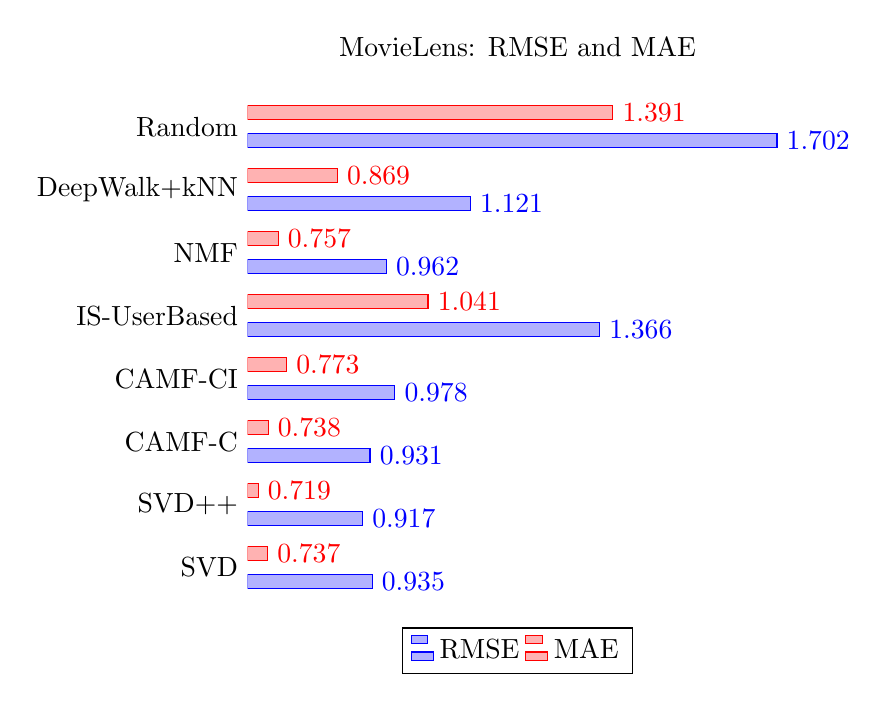
\begin{tikzpicture}
\begin{axis} [
    title    = {MovieLens: RMSE and MAE},
    xbar=5pt,
    /pgf/bar width=5pt,
    y axis line style = { opacity = 0 },
    axis x line       = none,
    tickwidth         = 0pt,
    enlarge x limits  = 0.02,
    ytick=data,
    y=0.8cm,
    nodes near coords={\pgfmathprintnumber[fixed zerofill, precision=3]{\pgfplotspointmeta}},
    legend style={at={(0.5,-0.03)}, anchor=north,legend columns=-1},
    symbolic y coords = {SVD,SVD++,CAMF-C,CAMF-CI,IS-UserBased,NMF,DeepWalk+kNN,Random},
  ]
\addplot coordinates{(0.935,SVD) (0.917,SVD++) (0.931,CAMF-C) (0.978,CAMF-CI) (1.366,IS-UserBased) (0.962,NMF) (1.121,DeepWalk+kNN) (1.702,Random)};
\addplot coordinates{(0.737,SVD) (0.719,SVD++) (0.738,CAMF-C) (0.773,CAMF-CI) (1.041,IS-UserBased) (0.757,NMF) (0.869,DeepWalk+kNN) (1.391,Random)};
\legend{RMSE,MAE}
\end{axis}
\end{tikzpicture}
\caption{RMSE and MAE results for MovieLens dataset across the investigated methods}
\label{graph:MLRMSEMAE}
\end{figure}

\begin{figure}[h]
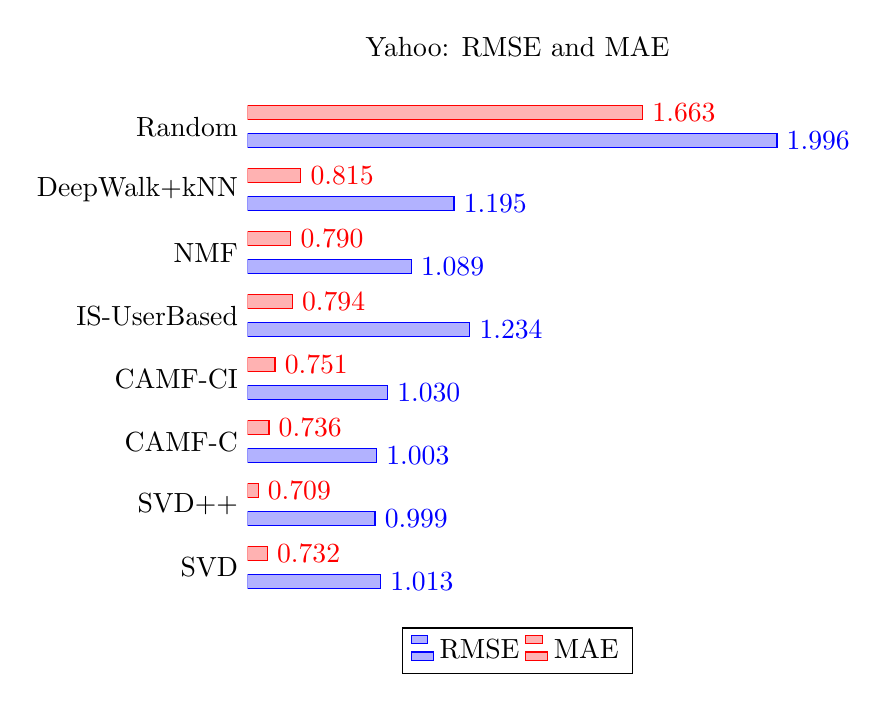
\begin{tikzpicture}
\begin{axis} [
    title    = {Yahoo: RMSE and MAE},
    xbar=5pt,
    /pgf/bar width=5pt,
    y axis line style = { opacity = 0 },
    axis x line       = none,
    tickwidth         = 0pt,
    enlarge x limits  = 0.02,
    ytick=data,
    y=0.8cm,
    nodes near coords={\pgfmathprintnumber[fixed zerofill, precision=3]{\pgfplotspointmeta}},
    legend style={at={(0.5,-0.03)}, anchor=north,legend columns=-1},
    symbolic y coords = {SVD,SVD++,CAMF-C,CAMF-CI,IS-UserBased,NMF,DeepWalk+kNN,Random},
  ]
\addplot coordinates{(1.013,SVD) (0.999,SVD++) (1.003,CAMF-C) (1.030,CAMF-CI) (1.234,IS-UserBased) (1.089,NMF) (1.195,DeepWalk+kNN) (1.996,Random)};
\addplot coordinates{(0.732,SVD) (0.709,SVD++) (0.736,CAMF-C) (0.751,CAMF-CI) (0.794,IS-UserBased) (0.790,NMF) (0.815,DeepWalk+kNN) (1.663,Random)};
\legend{RMSE,MAE}
\end{axis}
\end{tikzpicture}
\caption{RMSE and MAE results for Yahoo dataset across the investigated methods}
\label{graph:YahooRMSEMAE}
\end{figure}

\begin{figure}[h]
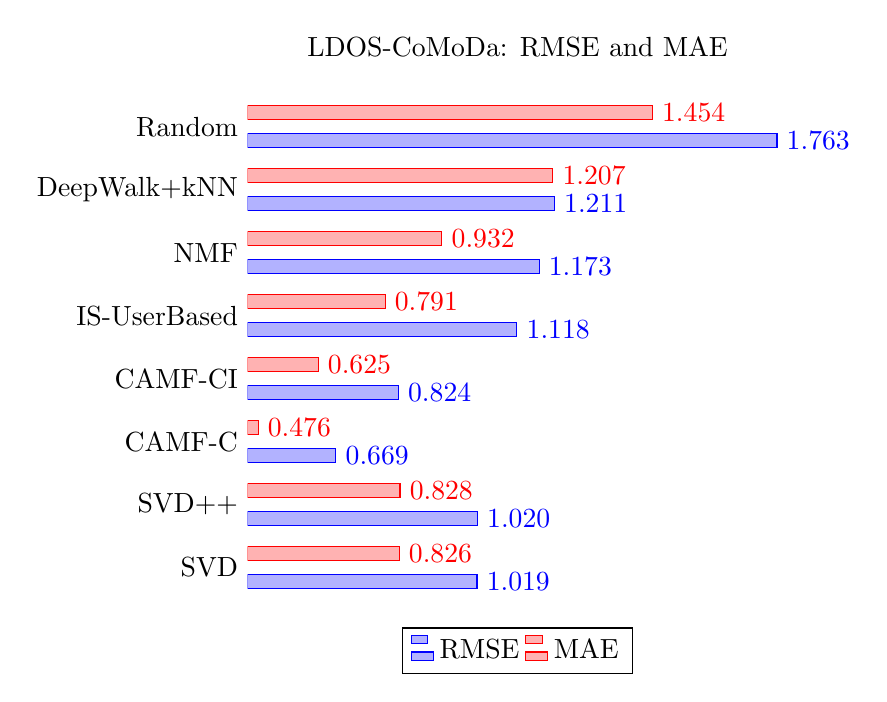
\begin{tikzpicture}
\begin{axis} [
    title    = {LDOS-CoMoDa: RMSE and MAE},
    xbar=5pt,
    /pgf/bar width=5pt,
    y axis line style = { opacity = 0 },
    axis x line       = none,
    tickwidth         = 0pt,
    enlarge x limits  = 0.02,
    ytick=data,
    y=0.8cm,
    nodes near coords={\pgfmathprintnumber[fixed zerofill, precision=3]{\pgfplotspointmeta}},
    legend style={at={(0.5,-0.03)}, anchor=north,legend columns=-1},
    symbolic y coords = {SVD,SVD++,CAMF-C,CAMF-CI,IS-UserBased,NMF,DeepWalk+kNN,Random},
  ]
\addplot coordinates{(1.019,SVD) (1.020,SVD++) (0.669,CAMF-C) (0.824,CAMF-CI) (1.118,IS-UserBased) (1.173,NMF) (1.211,DeepWalk+kNN) (1.763,Random)};
\addplot coordinates{(0.826,SVD) (0.828,SVD++) (0.476,CAMF-C) (0.625,CAMF-CI) (0.791,IS-UserBased) (0.932,NMF) (1.207,DeepWalk+kNN) (1.454,Random)};
\legend{RMSE,MAE}
\end{axis}
\end{tikzpicture}
\caption{RMSE and MAE results for LDOS-CoMoDa dataset across the investigated methods}
\label{graph:CoMoDaRMSEMAE}
\end{figure}

\begin{figure}[h]
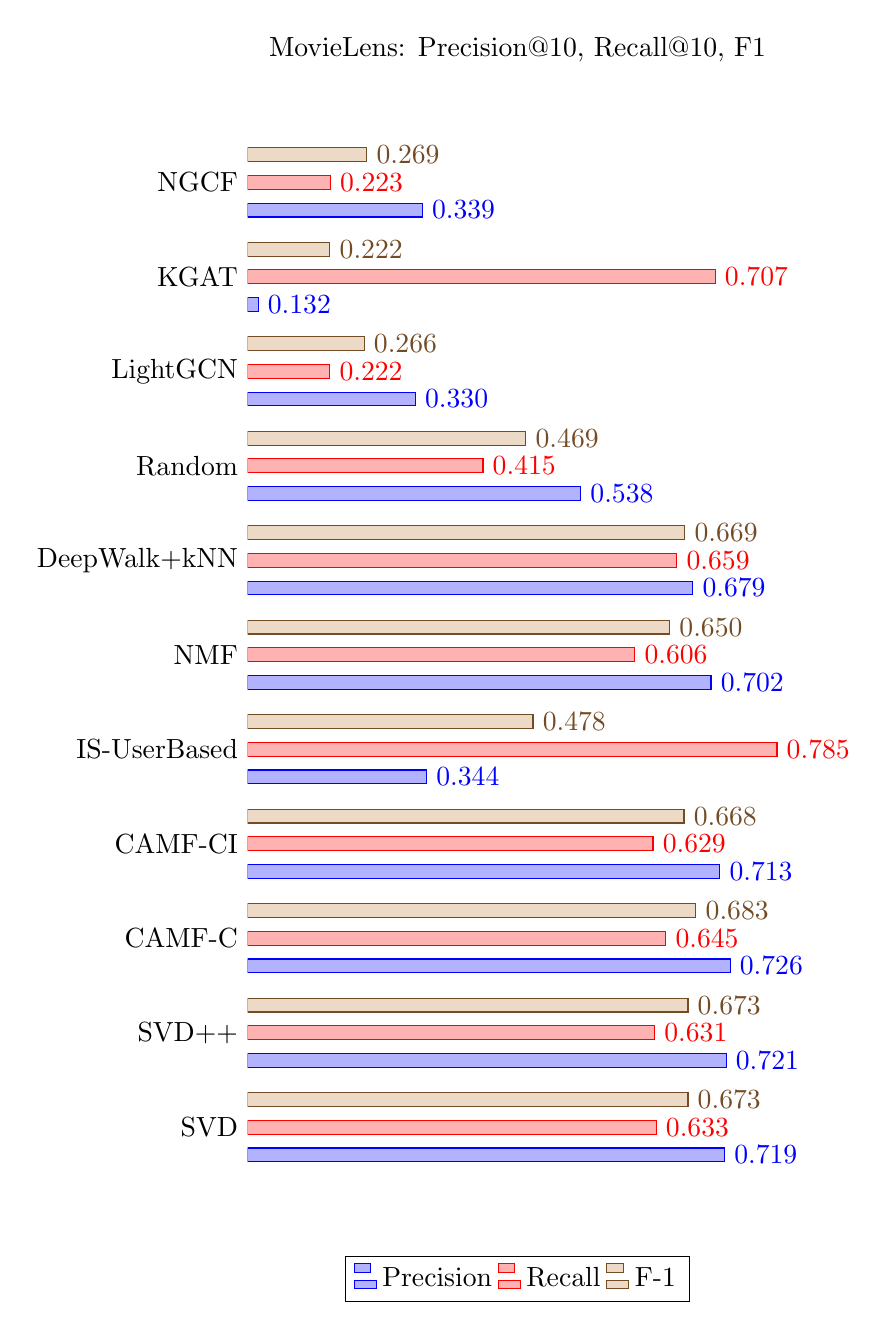
\begin{tikzpicture}
\begin{axis} [
    title    = {MovieLens: Precision@10, Recall@10, F1},
    xbar=5pt,
    /pgf/bar width=5pt,
    y axis line style = { opacity = 0 },
    axis x line       = none,
    tickwidth         = 0pt,
    enlarge x limits  = 0.02,
    ytick=data,
    y=1.2cm,
    nodes near coords={\pgfmathprintnumber[fixed zerofill, precision=3]{\pgfplotspointmeta}},
    legend style={at={(0.5,-0.03)}, anchor=north,legend columns=-1},
    symbolic y coords = {SVD,SVD++,CAMF-C,CAMF-CI,IS-UserBased,NMF,DeepWalk+kNN,Random,LightGCN,KGAT,NGCF},
  ]
\addplot coordinates{(0.719,SVD) (0.721,SVD++) (0.726,CAMF-C) (0.713,CAMF-CI) (0.344,IS-UserBased) (0.702,NMF) (0.679,DeepWalk+kNN) (0.538,Random) (0.3299,LightGCN) (0.1320,KGAT) (0.3386,NGCF)};
\addplot coordinates{(0.633,SVD) (0.631,SVD++) (0.645,CAMF-C) (0.629,CAMF-CI) (0.785,IS-UserBased) (0.606,NMF) (0.659,DeepWalk+kNN) (0.415,Random) (0.2222,LightGCN) (0.7072,KGAT) (0.2228,NGCF)};
\addplot coordinates{(0.673,SVD) (0.673,SVD++) (0.683,CAMF-C) (0.668,CAMF-CI) (0.478,IS-UserBased) (0.650,NMF) (0.669,DeepWalk+kNN) (0.469,Random) (0.265514,LightGCN) (0.222441,KGAT) (0.268757,NGCF)};
\legend{Precision,Recall,F-1}
\end{axis}
\end{tikzpicture}
\caption{Precision, recall and F1 results for MovieLens dataset across the investigated methods}
\label{graph:MLPrecRecF1}
\end{figure}

\begin{figure}[h]
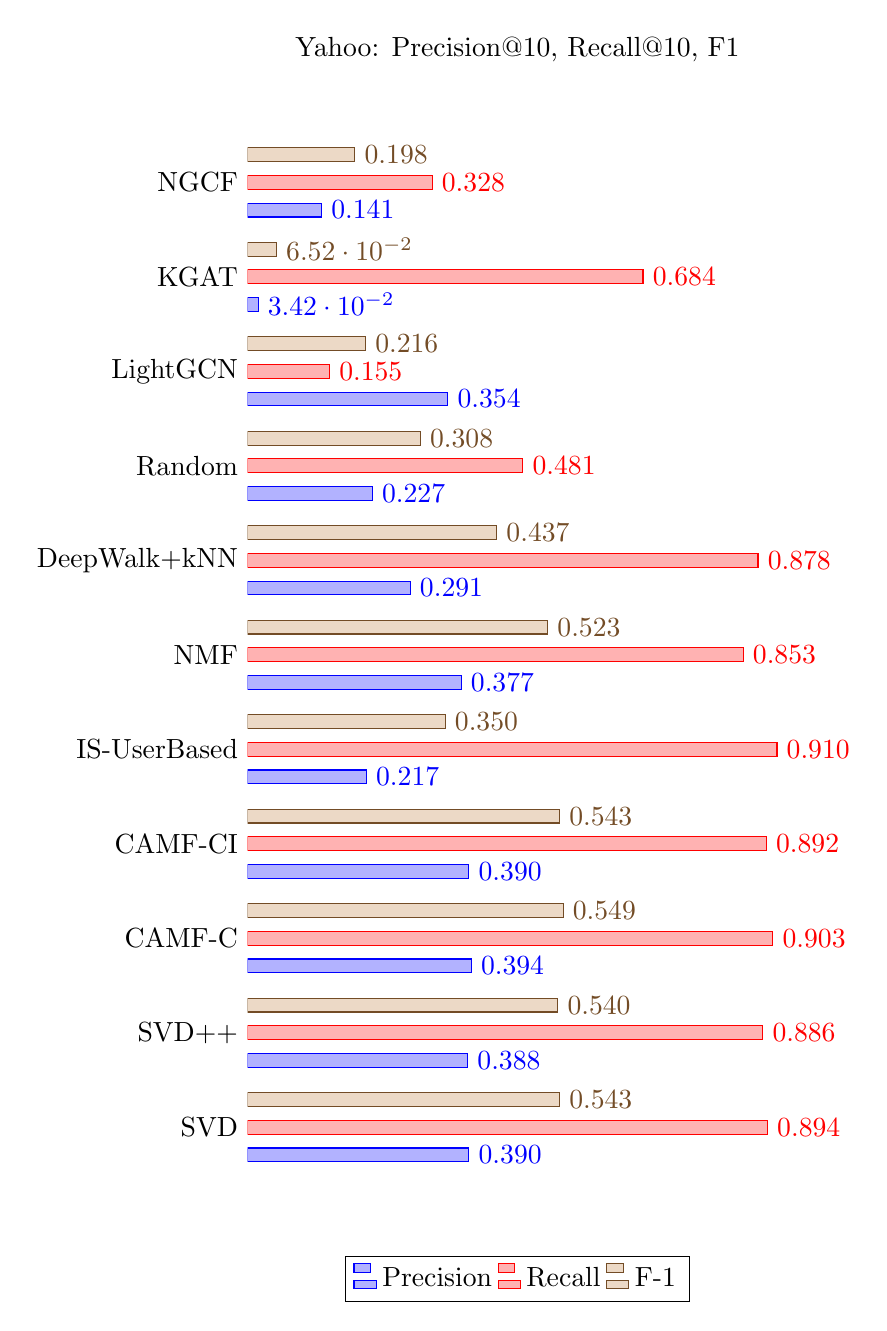
\begin{tikzpicture}
\begin{axis} [
    title    = {Yahoo: Precision@10, Recall@10, F1},
    xbar=5pt,
    /pgf/bar width=5pt,
    y axis line style = { opacity = 0 },
    axis x line       = none,
    tickwidth         = 0pt,
    enlarge x limits  = 0.02,
    ytick=data,
    y=1.2cm,
    nodes near coords={\pgfmathprintnumber[fixed zerofill, precision=3]{\pgfplotspointmeta}},
    legend style={at={(0.5,-0.03)}, anchor=north,legend columns=-1},
    symbolic y coords = {SVD,SVD++,CAMF-C,CAMF-CI,IS-UserBased,NMF,DeepWalk+kNN,Random,LightGCN,KGAT,NGCF},
  ]
\addplot coordinates{(0.390,SVD) (0.388,SVD++) (0.394,CAMF-C) (0.390,CAMF-CI) (0.217,IS-UserBased) (0.377,NMF) (0.291,DeepWalk+kNN) (0.227,Random) (0.3544,LightGCN) (0.0342,KGAT) (0.1414,NGCF)};
\addplot coordinates{(0.894,SVD) (0.886,SVD++) (0.903,CAMF-C) (0.892,CAMF-CI) (0.910,IS-UserBased) (0.853,NMF) (0.878,DeepWalk+kNN) (0.481,Random) (0.1548,LightGCN) (0.6840,KGAT) (0.3280,NGCF)};
\addplot coordinates{(0.543,SVD) (0.540,SVD++) (0.549,CAMF-C) (0.543,CAMF-CI) (0.350,IS-UserBased) (0.523,NMF) (0.437,DeepWalk+kNN) (0.308,Random) (0.2155,LightGCN) (0.0652,KGAT) (0.1976,NGCF)};
\legend{Precision,Recall,F-1}
\end{axis}
\end{tikzpicture}
\caption{Precision, recall and F1 results for Yahoo dataset across the investigated methods}
\label{graph:YahooPrecRecF1}
\end{figure}

\begin{figure}[h]
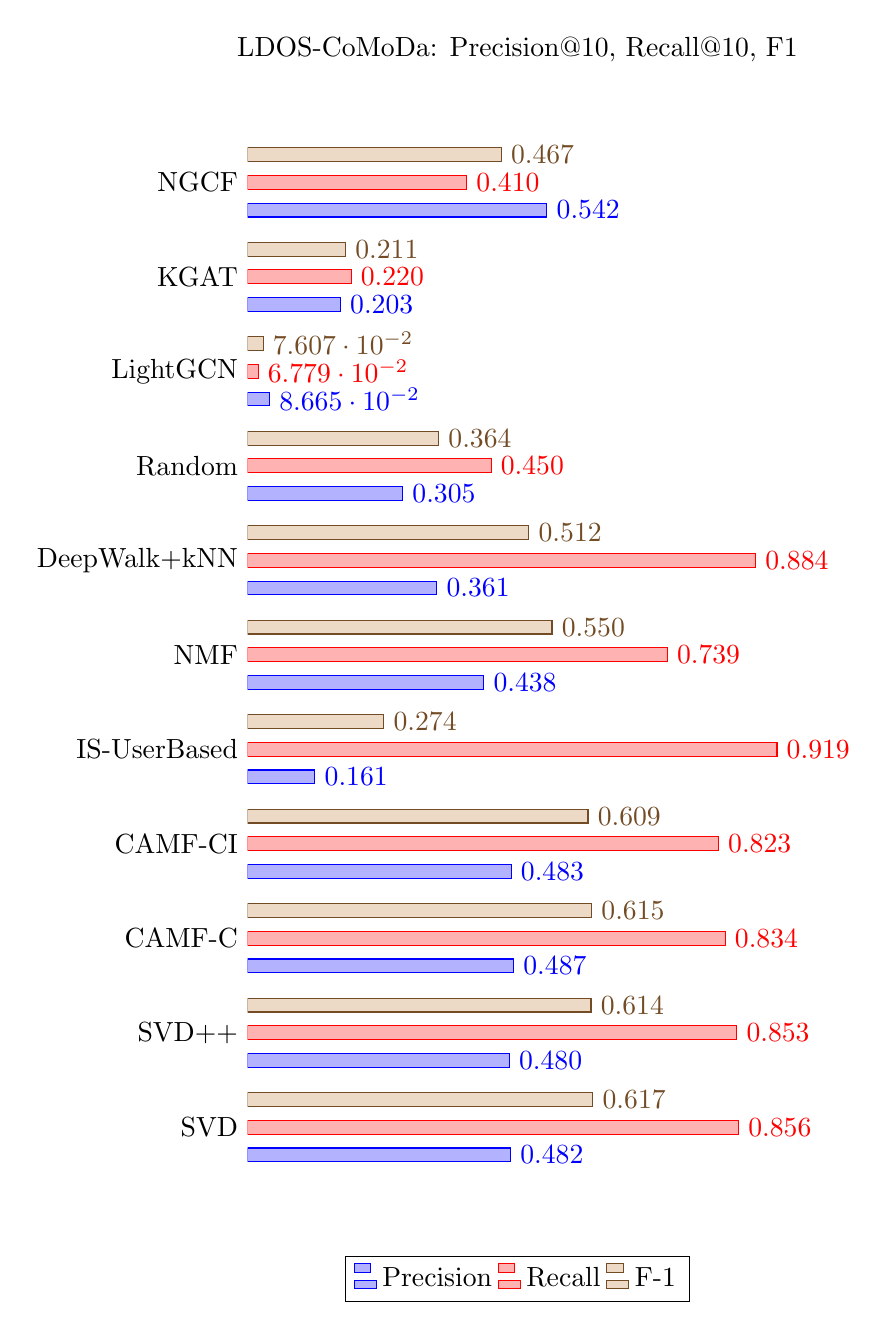
\begin{tikzpicture}
\begin{axis} [
    title    = {LDOS-CoMoDa: Precision@10, Recall@10, F1},
    xbar=5pt,
    /pgf/bar width=5pt,
    y axis line style = { opacity = 0 },
    axis x line       = none,
    tickwidth         = 0pt,
    enlarge x limits  = 0.02,
    ytick=data,
    y=1.2cm,
    nodes near coords={\pgfmathprintnumber[fixed zerofill, precision=3]{\pgfplotspointmeta}},
    legend style={at={(0.5,-0.03)}, anchor=north,legend columns=-1},
    symbolic y coords = {SVD,SVD++,CAMF-C,CAMF-CI,IS-UserBased,NMF,DeepWalk+kNN,Random,LightGCN,KGAT,NGCF},
  ]
\addplot coordinates{(0.482,SVD) (0.480,SVD++) (0.487,CAMF-C) (0.483,CAMF-CI) (0.161,IS-UserBased) (0.438,NMF) (0.361,DeepWalk+kNN) (0.305,Random) (0.08665008,LightGCN) (0.20284,KGAT) (0.5416,NGCF)};
\addplot coordinates{(0.856,SVD) (0.853,SVD++) (0.834,CAMF-C) (0.823,CAMF-CI) (0.919,IS-UserBased) (0.739,NMF) (0.884,DeepWalk+kNN) (0.450,Random) (0.067787792,LightGCN) (0.220396,KGAT) (0.41,NGCF)};
\addplot coordinates{(0.617,SVD) (0.614,SVD++) (0.615,CAMF-C) (0.609,CAMF-CI) (0.274,IS-UserBased) (0.550,NMF) (0.512,DeepWalk+kNN) (0.364,Random) (0.0760671,LightGCN) (0.211254,KGAT) (0.466700,NGCF)};
\legend{Precision,Recall,F-1}
\end{axis}
\end{tikzpicture}
\caption{Precision, recall and F1 results for LDOS-CoMoDa dataset across the investigated methods}
\label{graph:CoMoDaPrecRecF1}
\end{figure}

\begin{figure}[h]
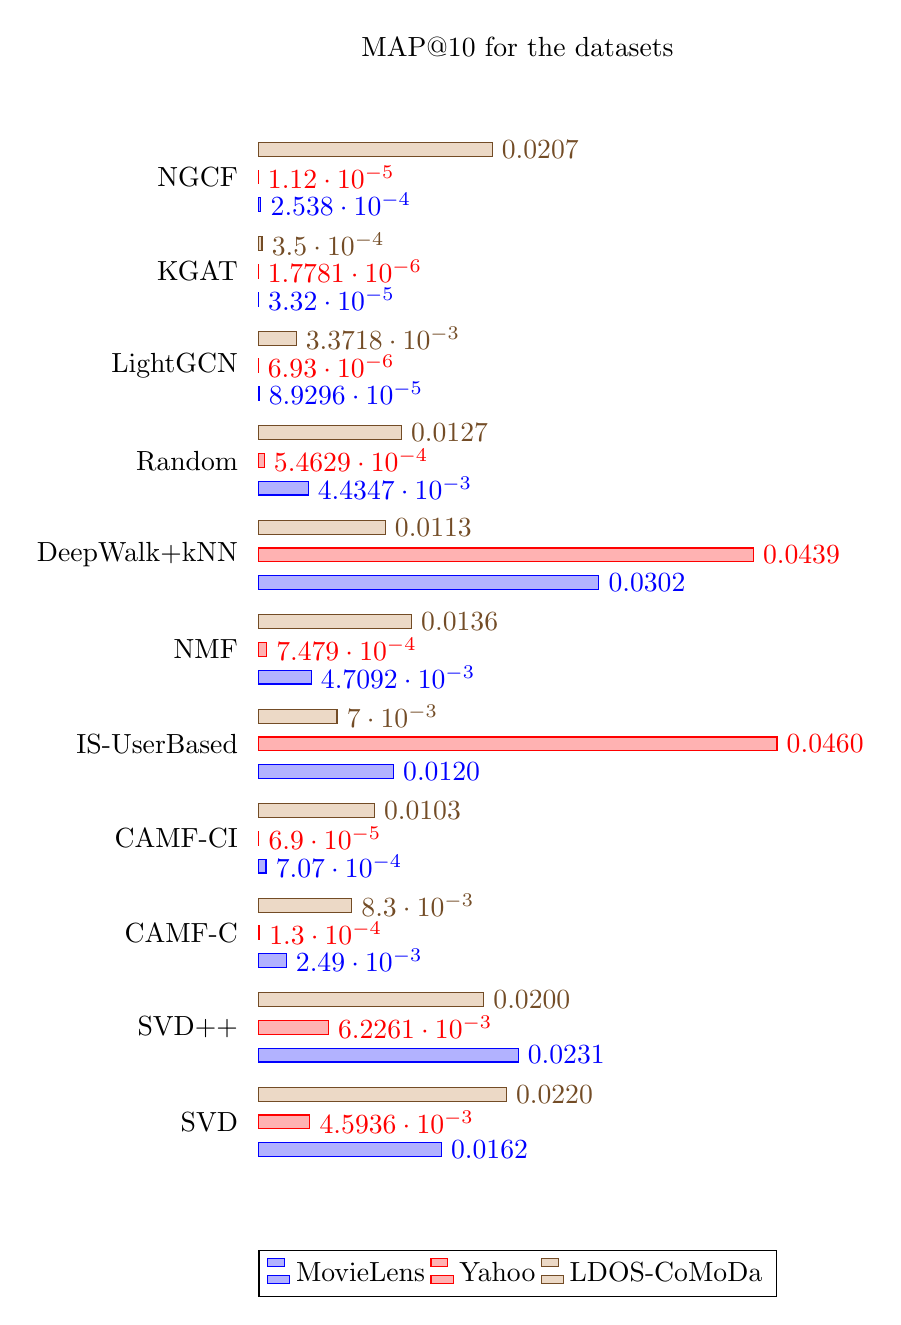
\begin{tikzpicture}
\begin{axis} [
    title    = {MAP@10 for the datasets},
    xbar=5pt,
    /pgf/bar width=5pt,
    y axis line style = { opacity = 0 },
    axis x line       = none,
    tickwidth         = 0pt,
    enlarge x limits  = 0.02,
    ytick=data,
    y=1.2cm,
    nodes near coords={\pgfmathprintnumber[fixed zerofill, precision=4]{\pgfplotspointmeta}},
    legend style={at={(0.5,-0.03)}, anchor=north,legend columns=-1},
    symbolic y coords = {SVD,SVD++,CAMF-C,CAMF-CI,IS-UserBased,NMF,DeepWalk+kNN,Random,LightGCN,KGAT,NGCF},
  ]
\addplot coordinates{(0.0162465951248284,SVD) (0.0230514217391177,SVD++) (0.00249,CAMF-C) (0.000707,CAMF-CI) (0.0120,IS-UserBased) (0.00470921880091866,NMF) (0.0302,DeepWalk+kNN) (0.00443467504522534,Random) (0.0000892961875081354,LightGCN) (0.0000332,KGAT) (0.0002538,NGCF)}; % MovieLens
\addplot coordinates{(0.00459364446058646,SVD) (0.00622607894470324,SVD++) (0.00013,CAMF-C) (0.000069,CAMF-CI) (0.046,IS-UserBased) (0.000747900814877045,NMF) (0.0439,DeepWalk+kNN) (0.000546288347257189,Random) (0.00000693,LightGCN) (0.0000017781423399345,KGAT) (0.0000112,NGCF)}; % Yahoo
\addplot coordinates{(0.022,SVD) (0.02,SVD++) (0.0083,CAMF-C) (0.0103,CAMF-CI) (0.007,IS-UserBased) (0.0136,NMF) (0.01127,DeepWalk+kNN) (0.0126990696917064,Random) (0.00337181254,LightGCN) (0.00035,KGAT) (0.020748,NGCF)}; % CoMoDa
\legend{MovieLens,Yahoo,LDOS-CoMoDa}
\end{axis}
\end{tikzpicture}
\caption{MAP@10 results for the dataset across the investigated methods}
\label{graph:MAP10}
\end{figure}

\begin{figure}[h]
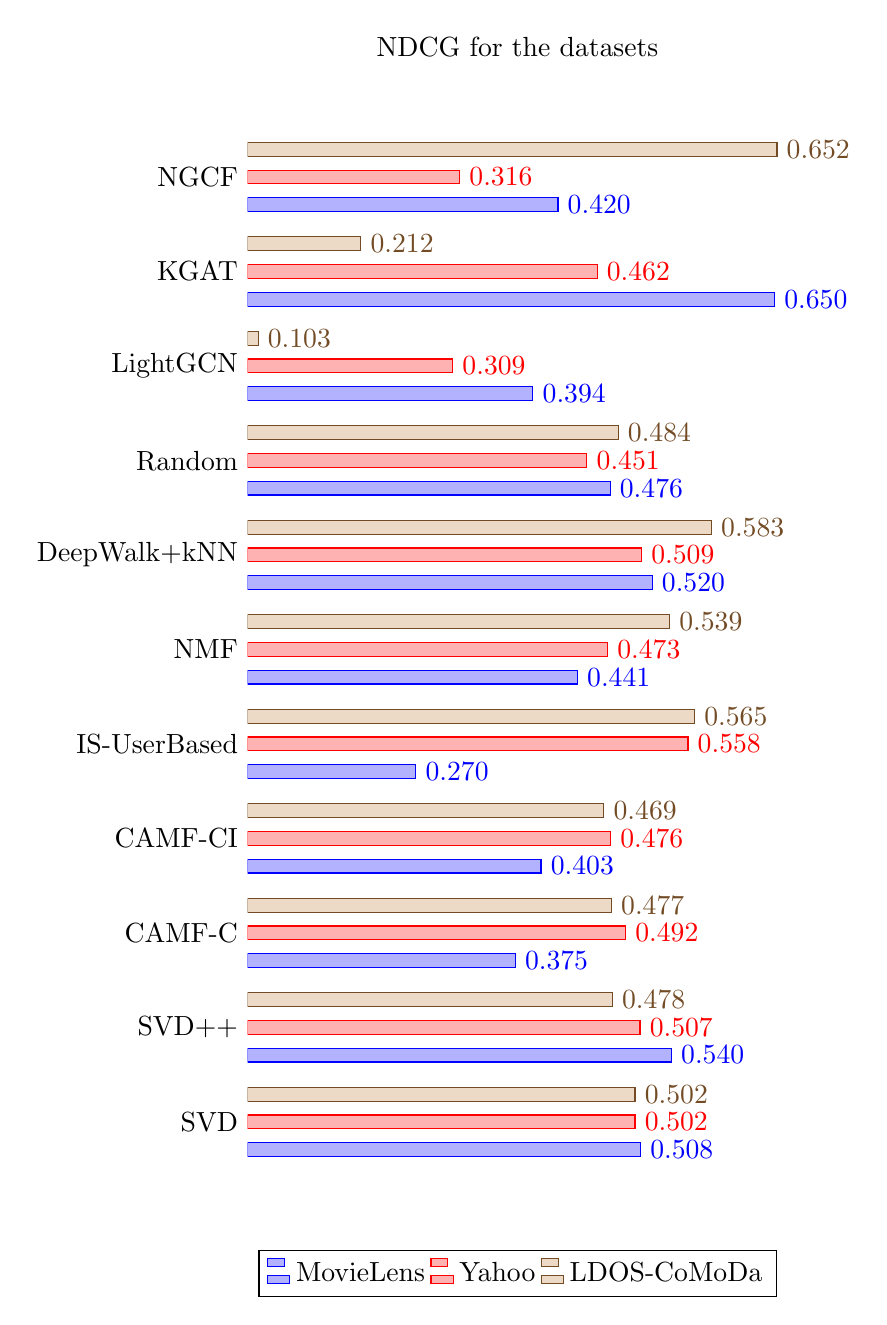
\begin{tikzpicture}
\begin{axis} [
    title    = {NDCG for the datasets},
    xbar=5pt,
    /pgf/bar width=5pt,
    y axis line style = { opacity = 0 },
    axis x line       = none,
    tickwidth         = 0pt,
    enlarge x limits  = 0.02,
    ytick=data,
    y=1.2cm,
    nodes near coords={\pgfmathprintnumber[fixed zerofill, precision=3]{\pgfplotspointmeta}},
    legend style={at={(0.5,-0.03)}, anchor=north,legend columns=-1},
    symbolic y coords = {SVD,SVD++,CAMF-C,CAMF-CI,IS-UserBased,NMF,DeepWalk+kNN,Random,LightGCN,KGAT,NGCF},
  ]
\addplot coordinates{(0.507788476243958,SVD) (0.540462250066491,SVD++) (0.3752,CAMF-C) (0.4025,CAMF-CI) (0.270,IS-UserBased) (0.441025641977599,NMF) (0.5201,DeepWalk+kNN) (0.475627993916583,Random) (0.3939,LightGCN) (0.6497,KGAT) (0.4204,NGCF)}; % MovieLens
\addplot coordinates{(0.501928001717915,SVD) (0.507223962441533,SVD++) (0.492,CAMF-C) (0.476,CAMF-CI) (0.558,IS-UserBased) (0.472880077638768,NMF) (0.5089,DeepWalk+kNN) (0.451040991988228,Random) (0.3090,LightGCN) (0.4618,KGAT) (0.3164,NGCF)}; % Yahoo
\addplot coordinates{(0.502,SVD) (0.478,SVD++) (0.477,CAMF-C) (0.469,CAMF-CI) (0.565,IS-UserBased) (0.5385,NMF) (0.5828,DeepWalk+kNN) (0.484100128099788,Random) (0.103,LightGCN) (0.21176,KGAT) (0.6522,NGCF) }; % CoMoDa
\legend{MovieLens,Yahoo,LDOS-CoMoDa}
\end{axis}
\end{tikzpicture}
\caption{NDCG@10 results for the dataset across the investigated methods}
\label{graph:NDCG10}
\end{figure}

